%%% This file contains the third  report. It cannot be compiled on it's own.

%{{{ Versuch 3

\setcounter{section}{3}
\addsec{Versuch 3}
%{{{
Der dritte Versuch beschäftigte sich mit Oszilloskopen und ihren Tücken.
%}}}

%{{{
\subsection{Signalerfassung und Artefakte}
In diesem Versuch wurde das DSO direkt mit dem Signalgenerator verbunden. Dort ergab sich schon das erste Problem: Laut Anleitung sollte die Zeitbasis auf 0,2ms/Skt eingestellt werden, doch das DSO unterstützt diese Einstellung nicht. Stattdessen habe ich 0,25ms/Skt verwendet.
Der Signalgenerator wurde auf 1 kHz gestellt.\\

\begin{tabular}{|l|l|}
	\hline
	Zeitbasis &  Schwingungen \\
	\hline
	\hline
	0,1 ms = 100 \mu s & 1\\
	\hline
	0,25 ms = 250 \mu s & 2.5\\
	\hline
	0,5 ms = 50 \mu s & 5\\
	\hline
	1 ms & 10 \\
	\hline
\end{tabular}
\vspace{0.5cm}

Bei 1V/Skt ist die Amplitude der Signalschwingung 4 Skalenteile. Somit wird die angelegte Spannung mit 4 V bemessen. Dies entspricht der Einstellung des Signalgenerators.
\begin{figure}[H]
	\centering
	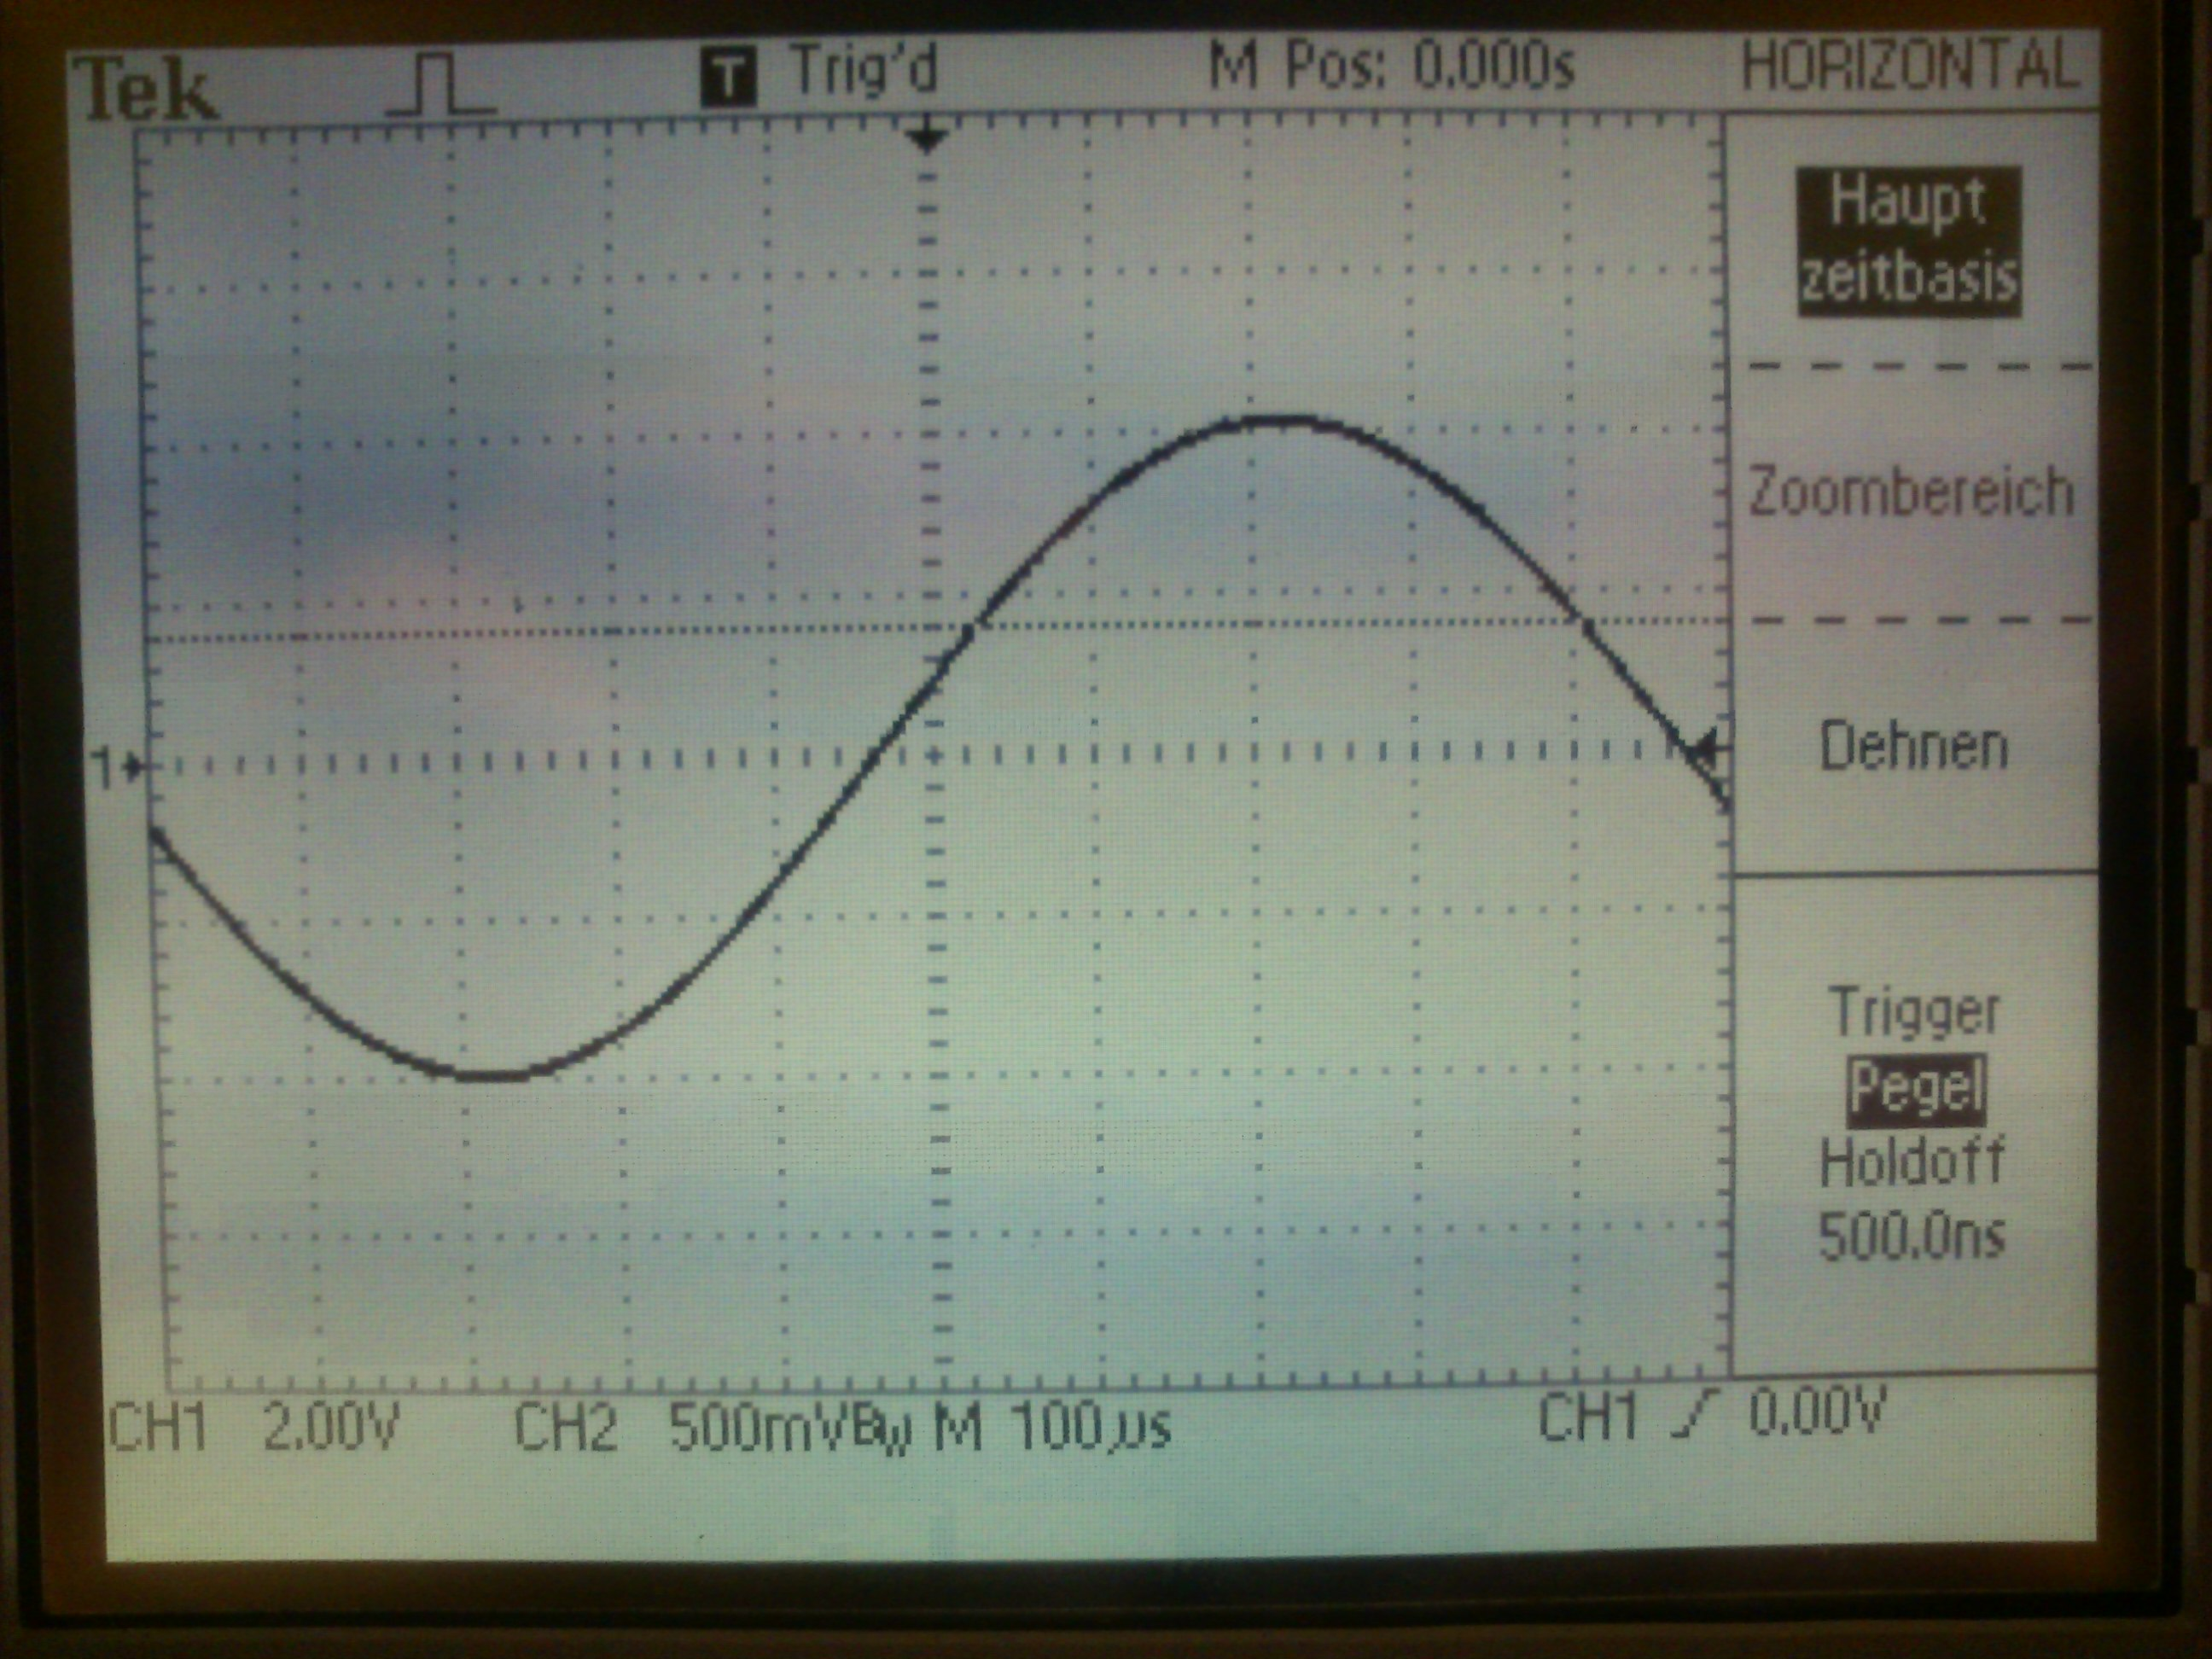
\includegraphics[width=\linewidth]{versuch3/oszi/DSC_0240.JPG}
	\caption{Sinusspannung durch Verstellen von Triggerlevel und Verzögerung mittig zentriert}
\end{figure}
\begin{figure}[H]
	\centering
	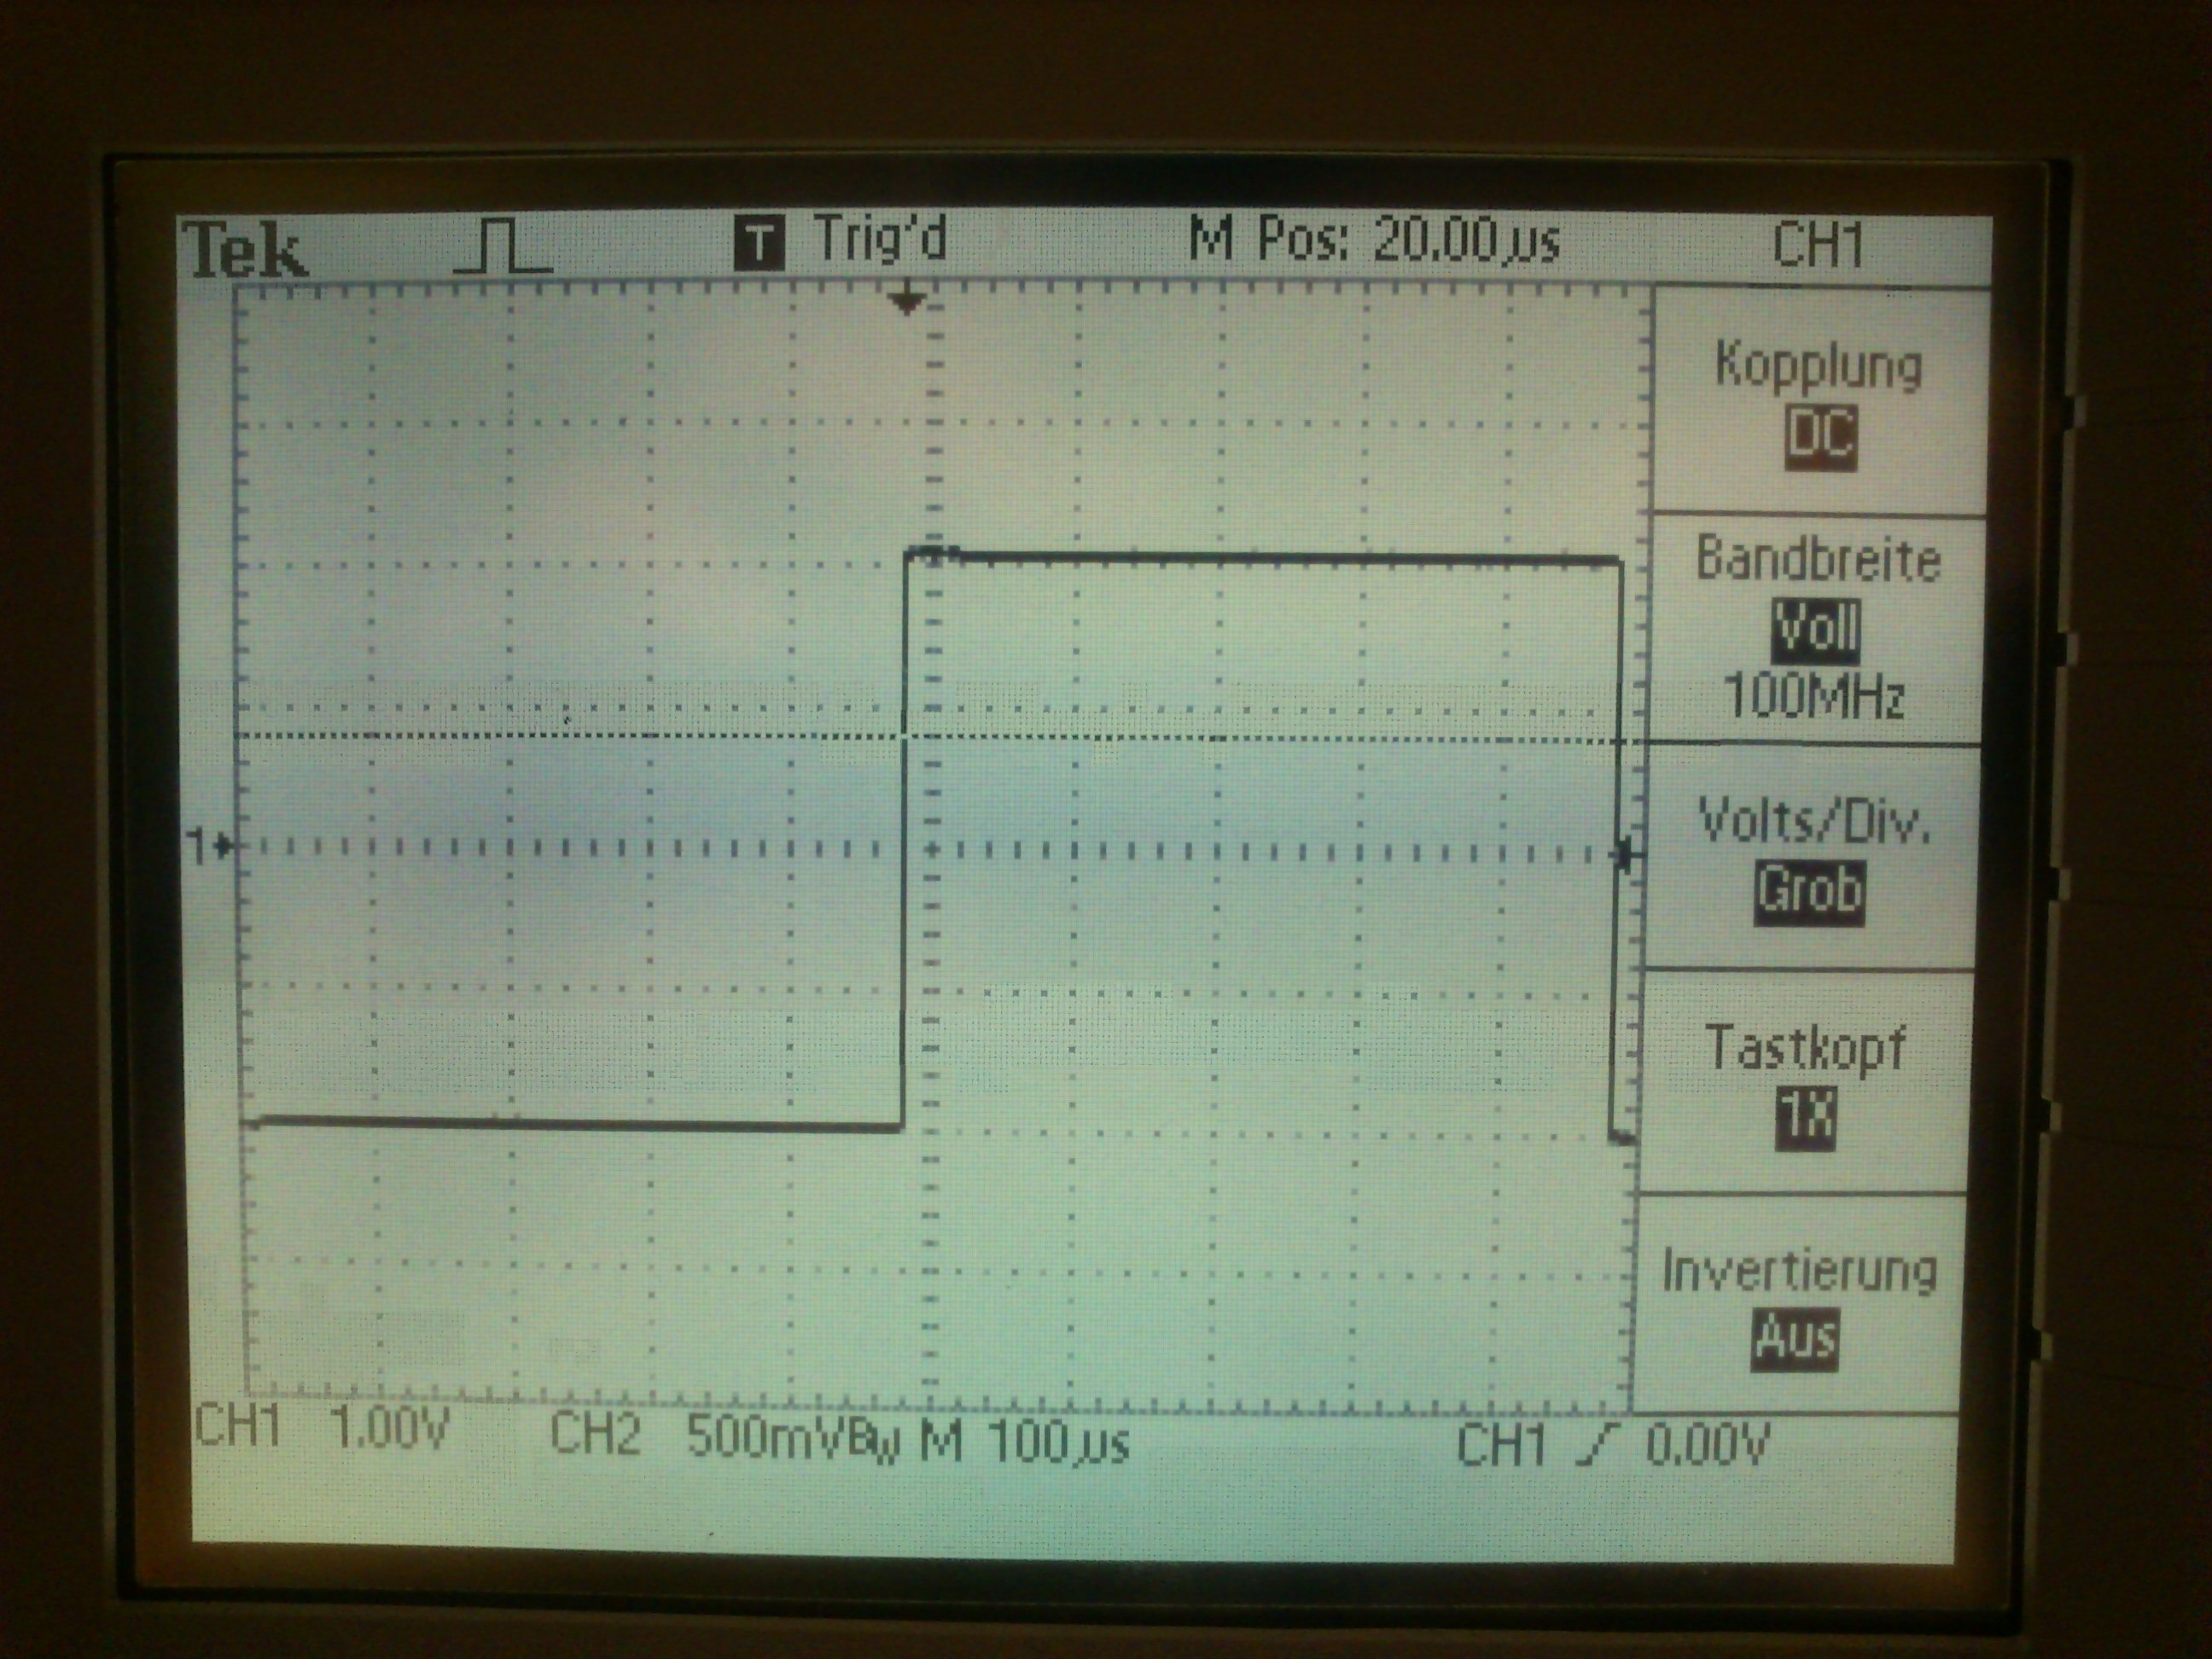
\includegraphics[width=\linewidth]{versuch3/oszi/DSC_0246.JPG}
	\caption{Eine Rechteckspannung}
\end{figure}
\begin{figure}[H]
	\centering
	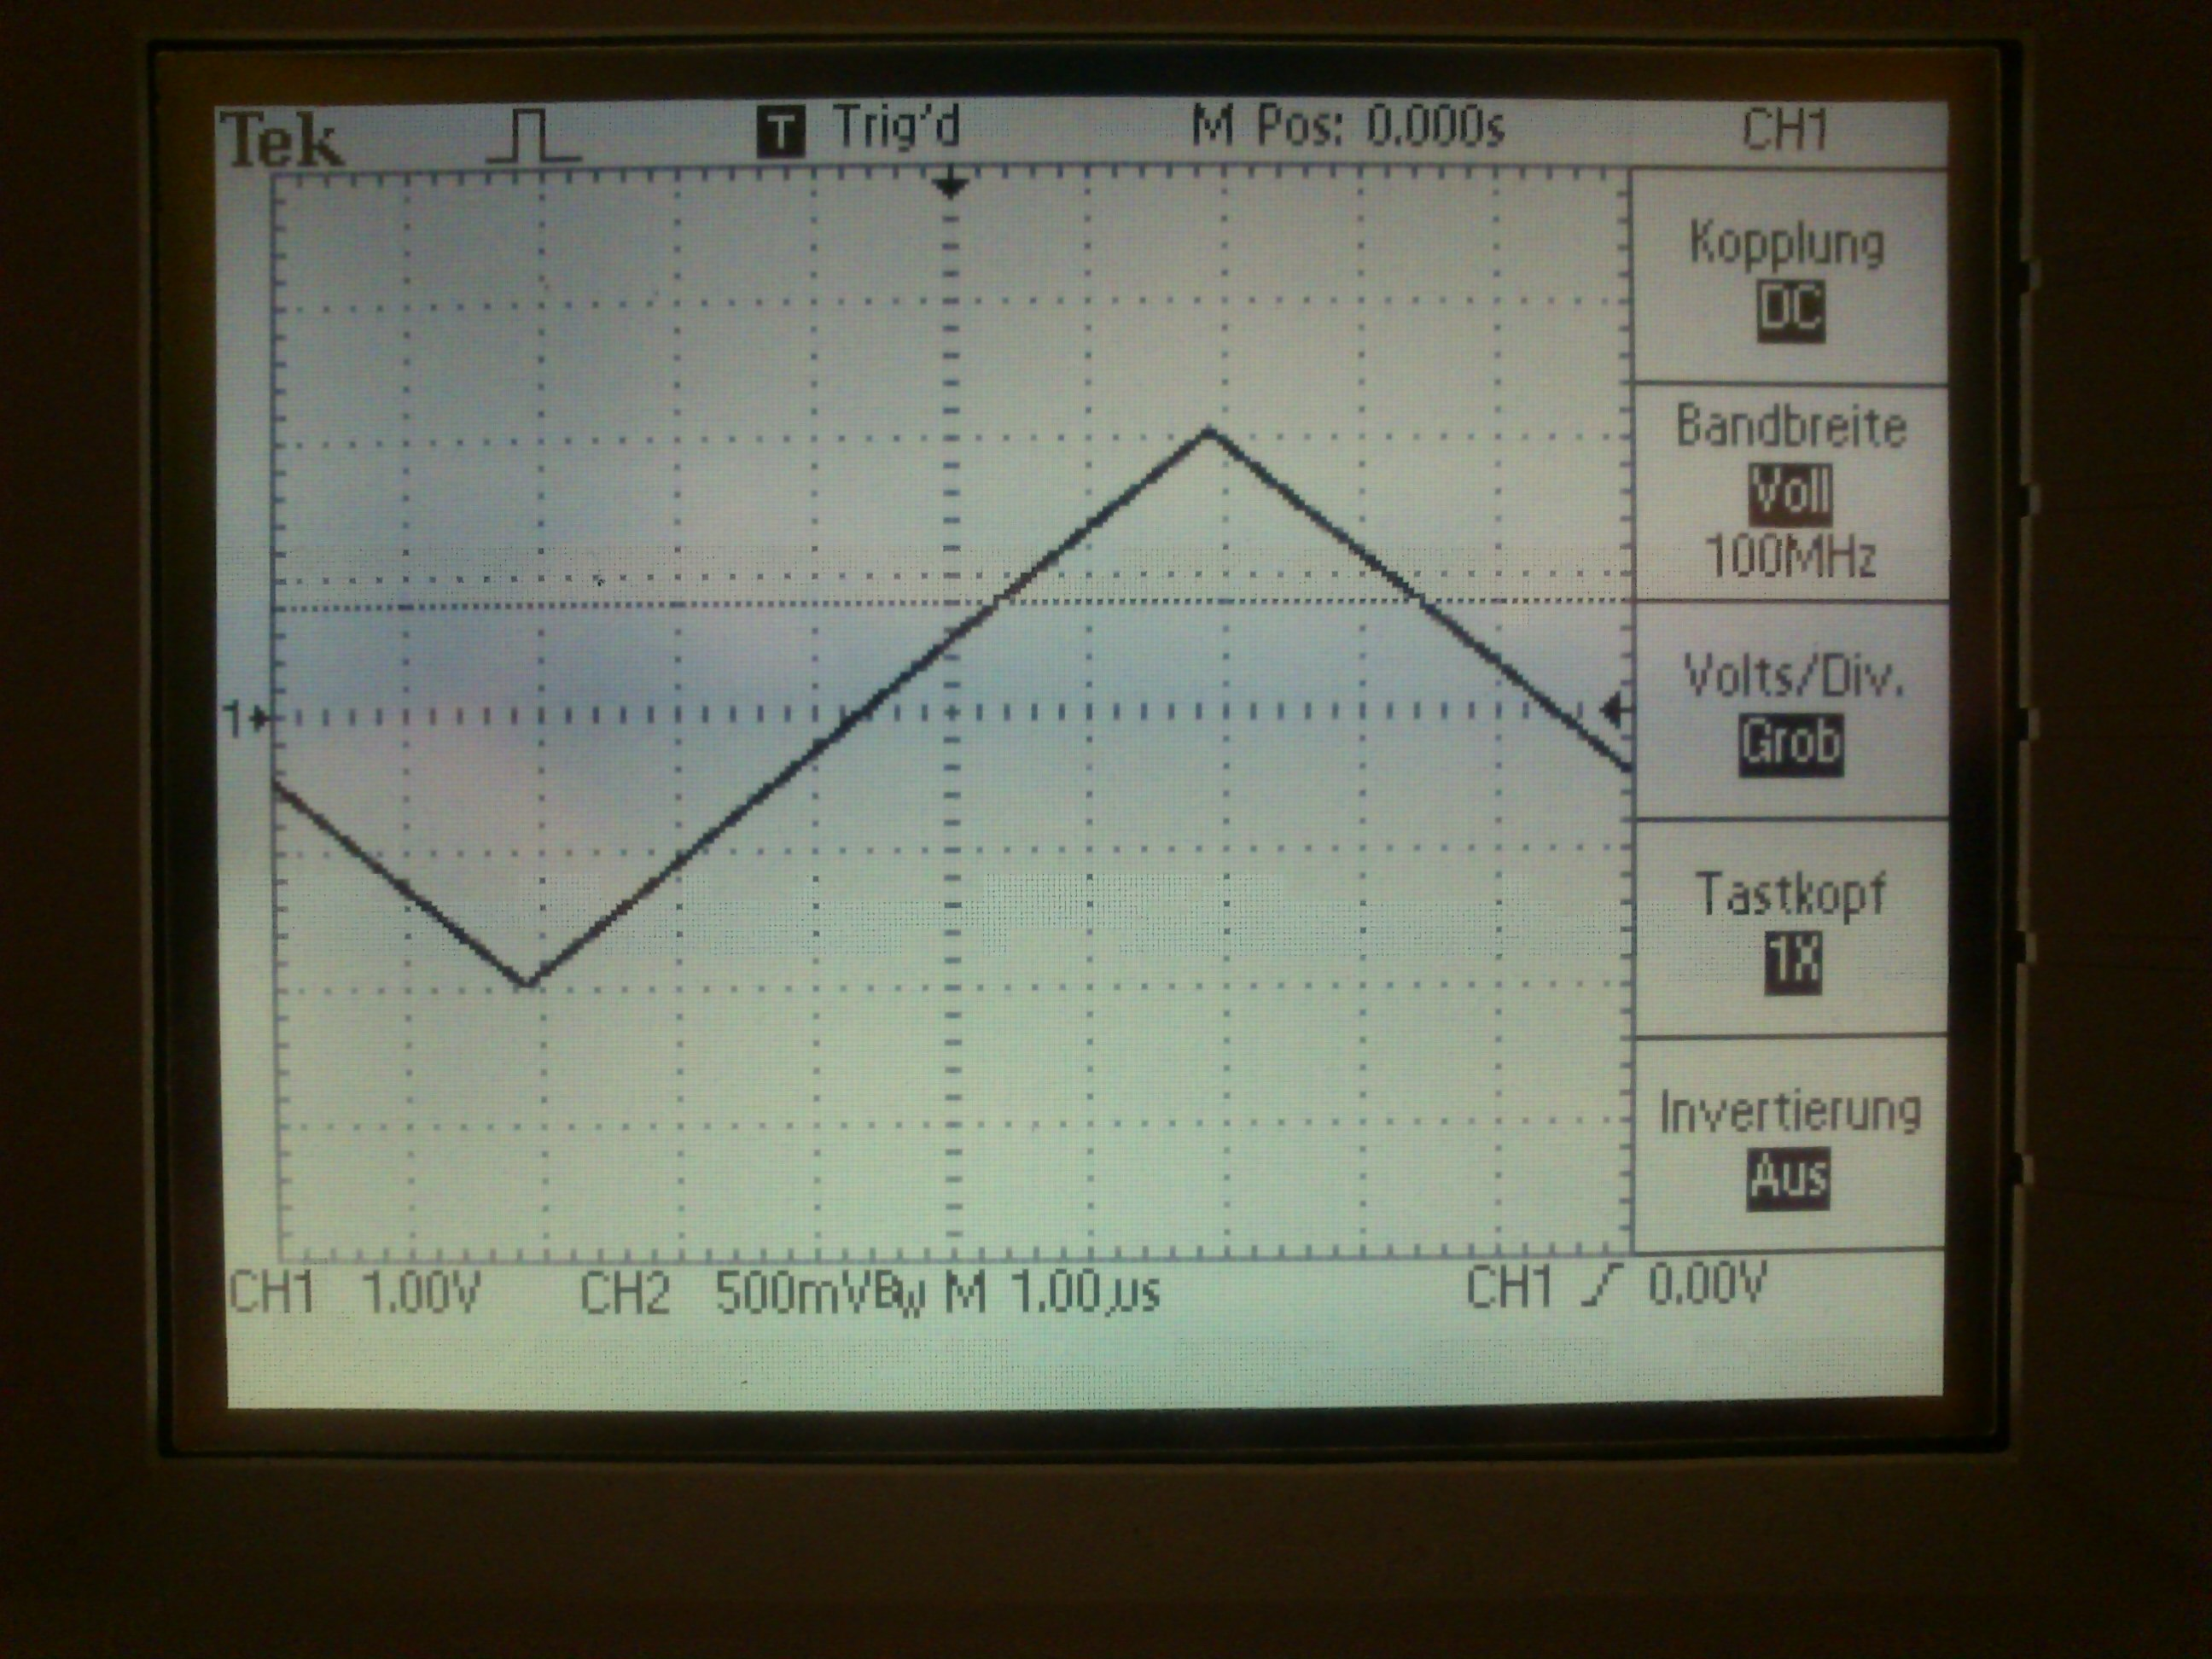
\includegraphics[width=\linewidth]{versuch3/oszi/DSC_0252.JPG}
	\caption{Und eine Dreieckspannung}
\end{figure}

Als nächstes wurde der Generator auf 1 MHz Sinus gestellt und mit dem Oszilloskop bei einer Zeitbasis von 1 µS die Frequenz gemessen:
\begin{figure}[H]
	\centering
	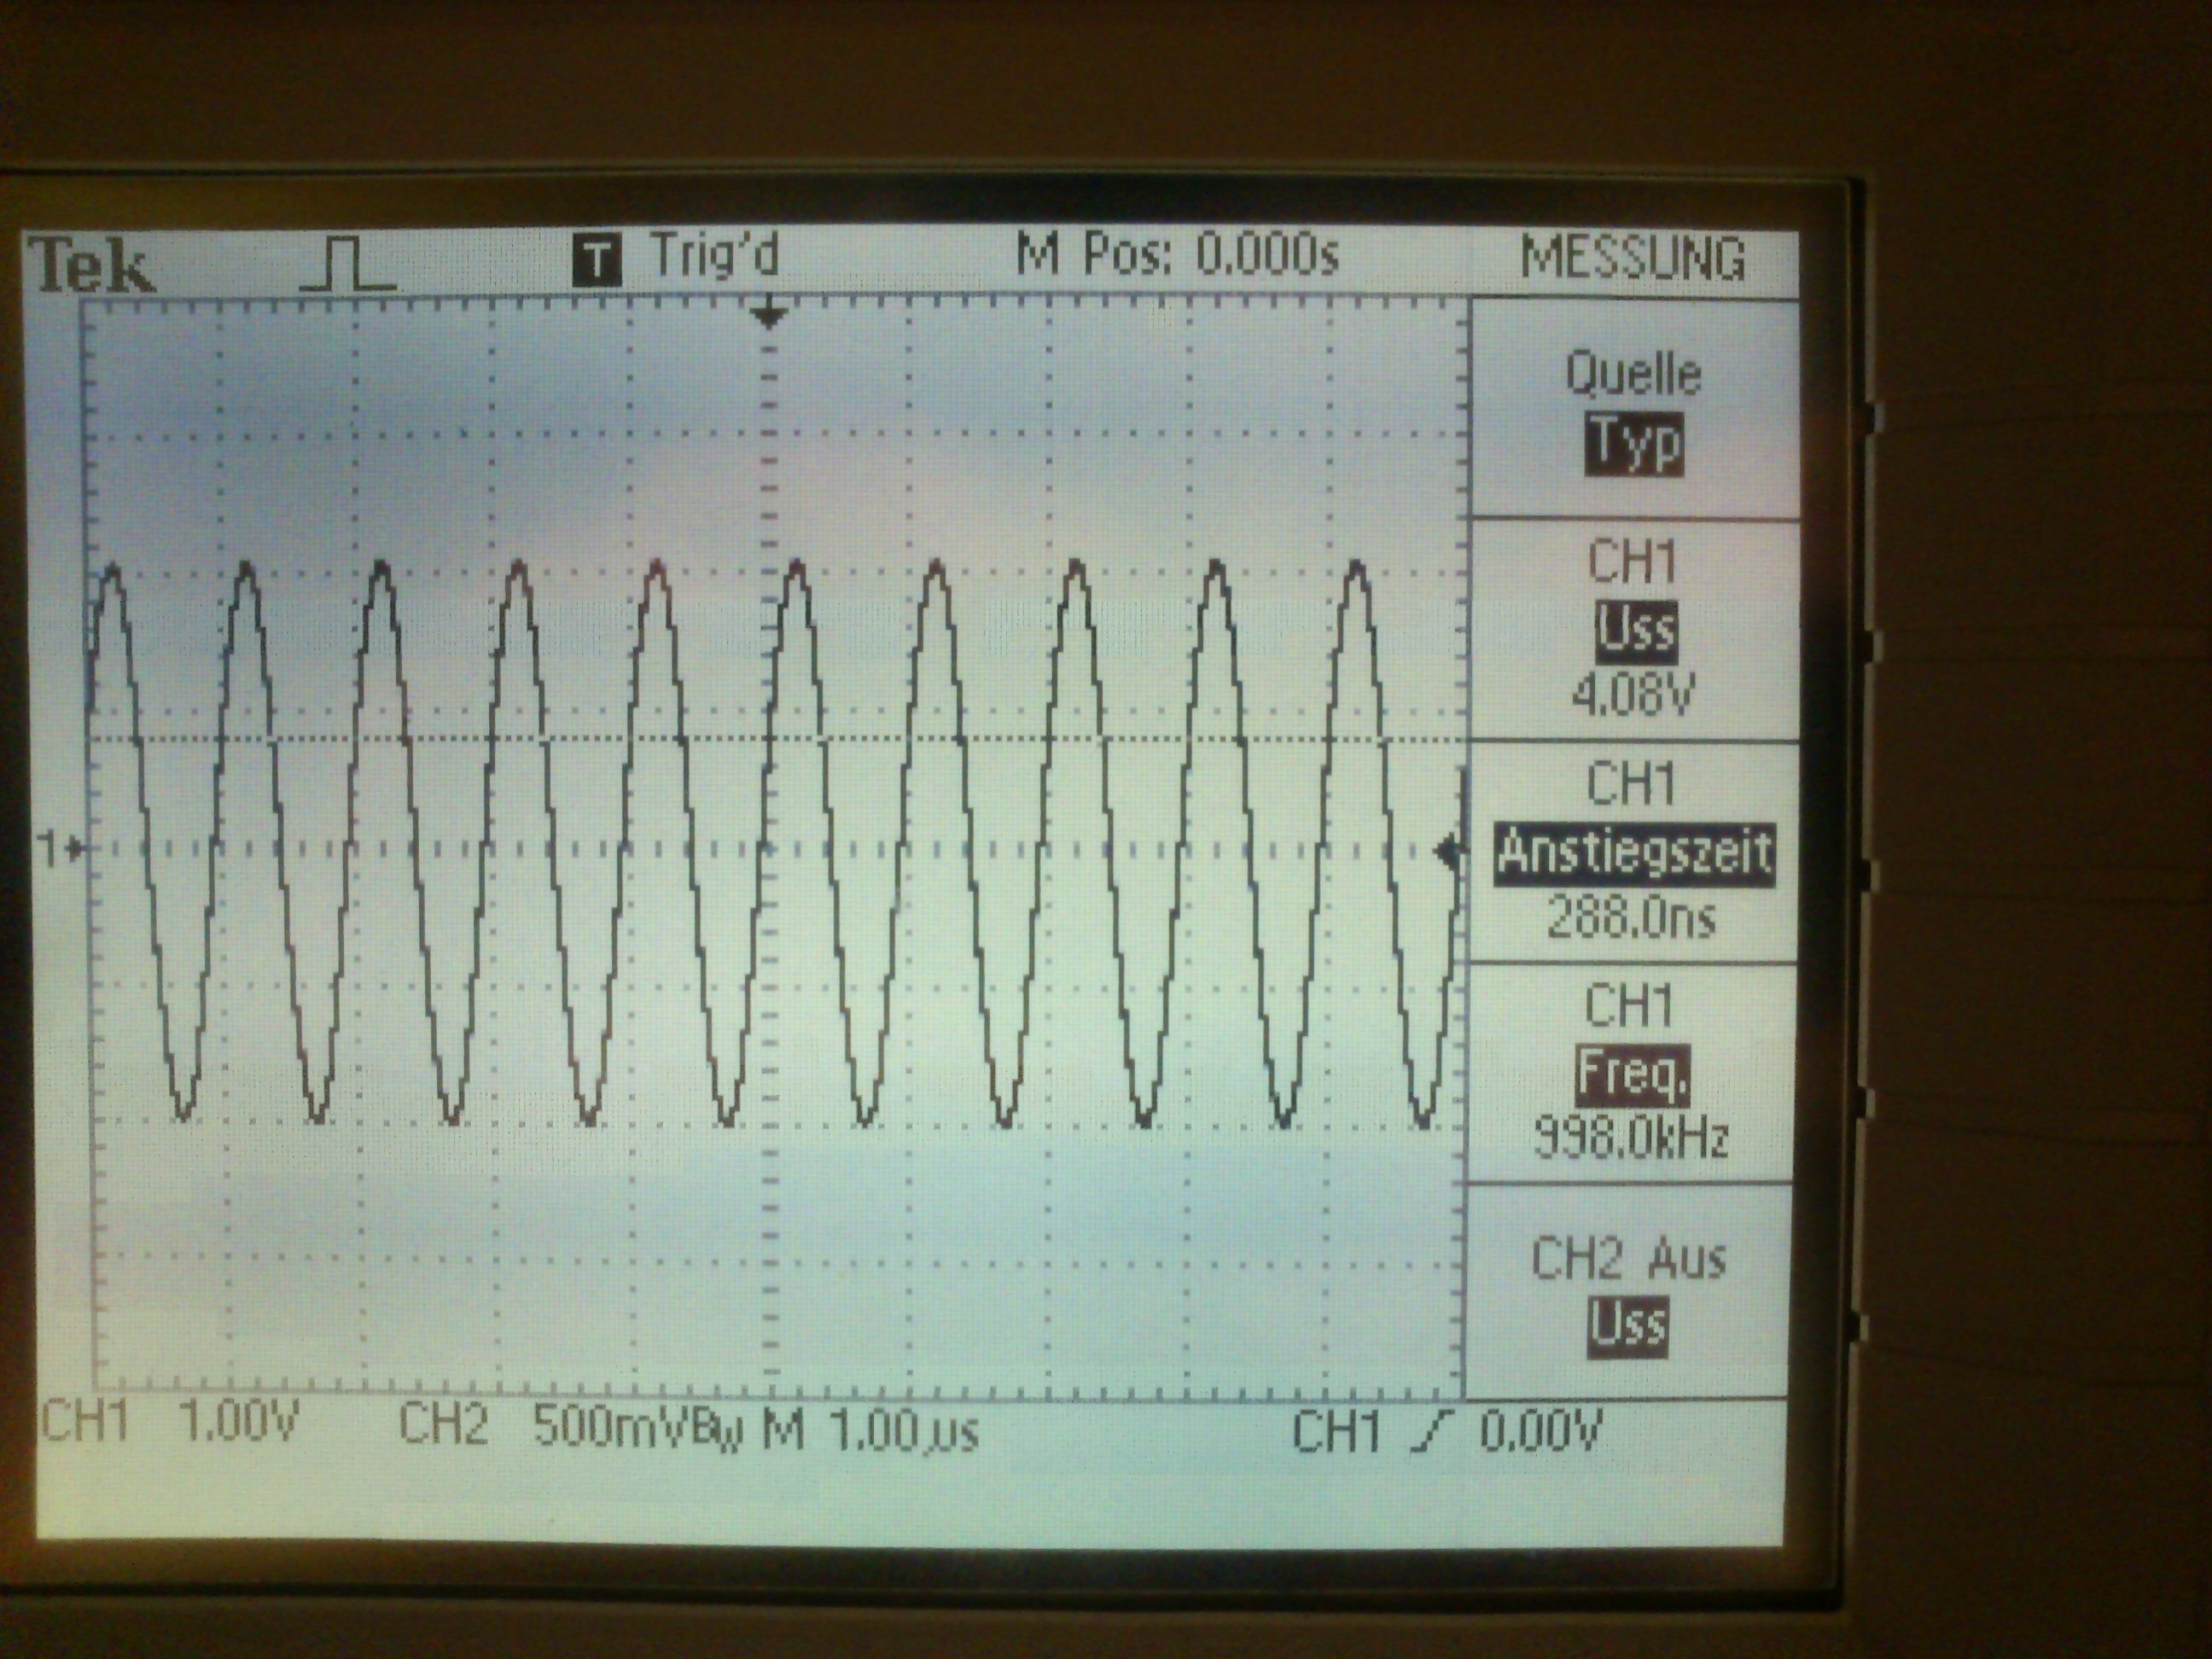
\includegraphics[width=\linewidth]{versuch3/oszi/DSC_0253.JPG}
	\caption{Frequenzmessung bei 1 MHz und 1µs Zeitbasis}
\end{figure}
Und dann die Messung bei einer Zeitbasis von 25 ms wiederholt:
\begin{figure}[H]
	\centering
	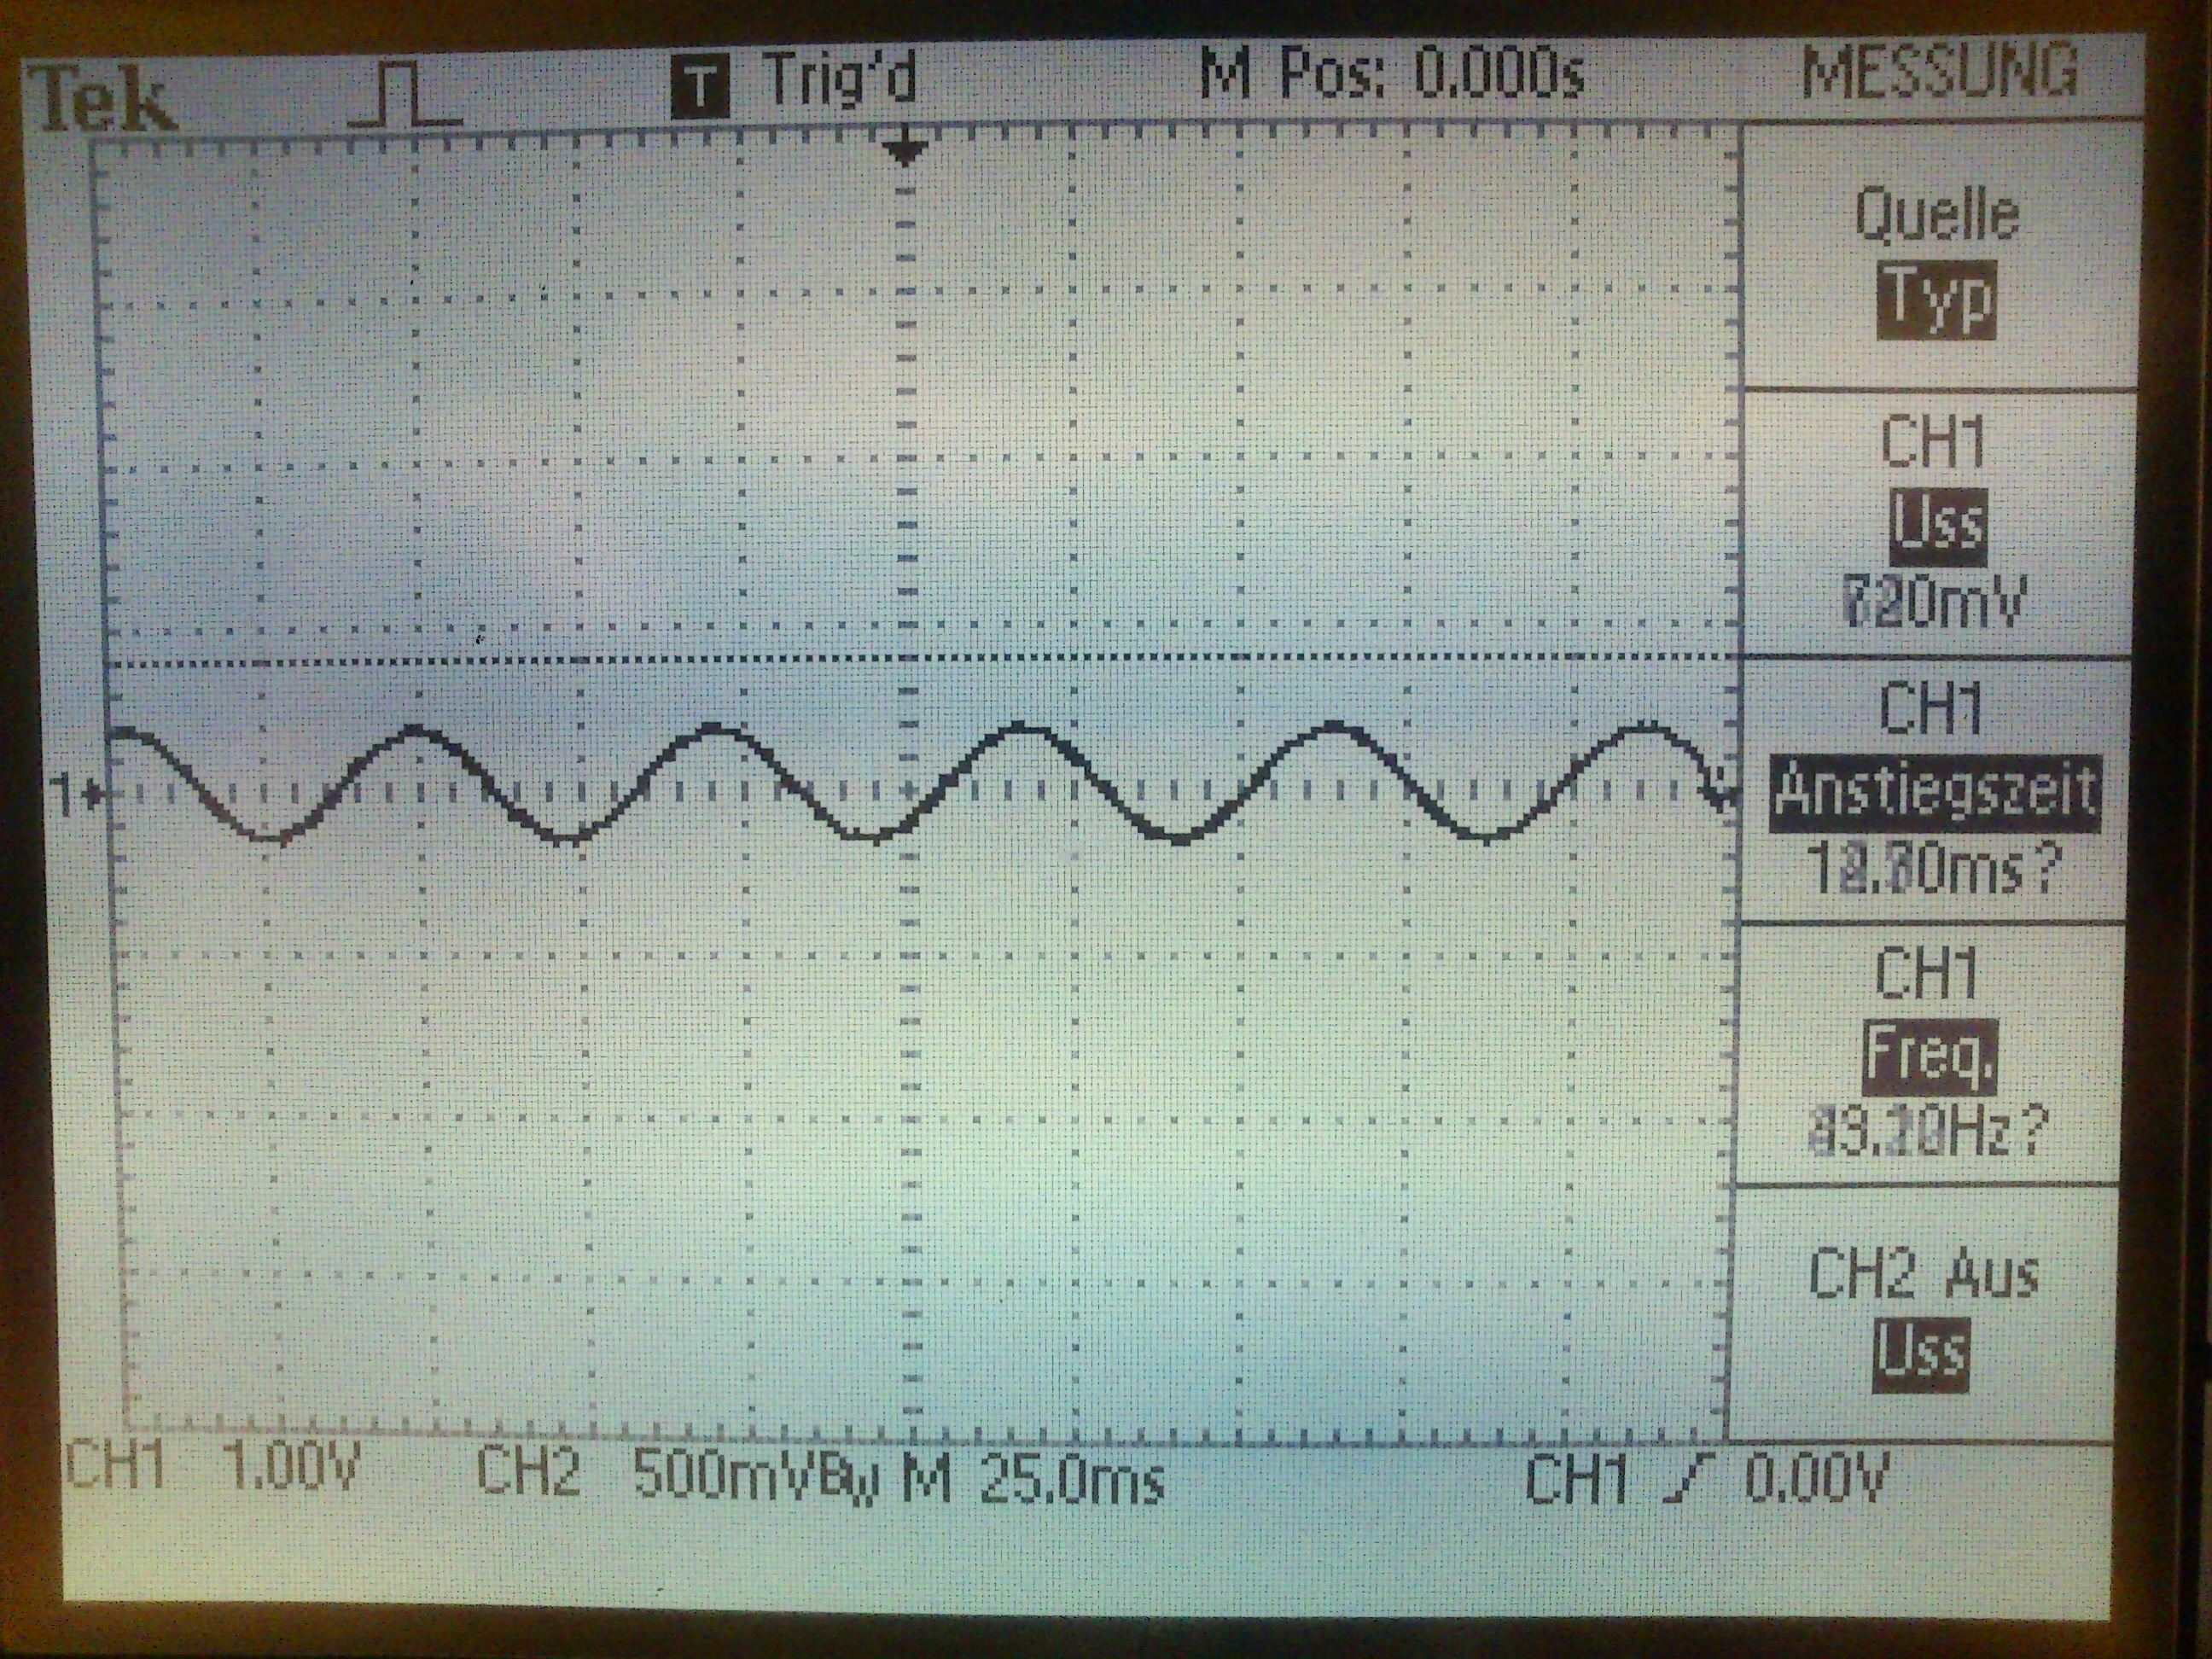
\includegraphics[width=\linewidth]{versuch3/oszi/DSC_0254.JPG}
	\caption{Frequenzmessung bei 1 MHz und 25 ms Zeitbasis}
\end{figure}
Es wird ein völlig falsches Signal angezeigt. Es ist zwar ein Sinus, aber die Frequenz und Amplitude stimmen nicht. Dies liegt daran, dass das Oszilloskop eigentlich nicht genug Messpunkte liefert, um jede Schwingung exakt auszumessen (Stichwort Nyquist-Frequenz, Shannon-Kriterium). Die angezeigte Freqyenz ist 43,1 Hz. Leider konnte ich hiervon kein sauberes Bild schießen, da die Anzeige zu stark schwankte.
%}}}

%{{{
\subsection{Aufbau eines Oszilators mit NE555}
Zuerst sollte die Frequenz des Oszillators bestimmt werden:\\
$ f=\frac{1}{T},\; T = 0,693 * (R_A + 2 R_B) * C;\; Ra = 1kΩ,\; Rb = 1kΩ,\; C = 4.7nF$\\
$\Rightarrow f=\frac{1}{0,693 * (1kΩ + 2*1kΩ) * 4.7nF} = 102.35 kHz$\\
Als Nächstes habe ich die Frequenz mit dem Oszilloskop zu 88.75 kHz ermittelt. Vermutlich kommt die Differenz von Bauteilschwankungen.
\begin{figure}[H]
	\centering
	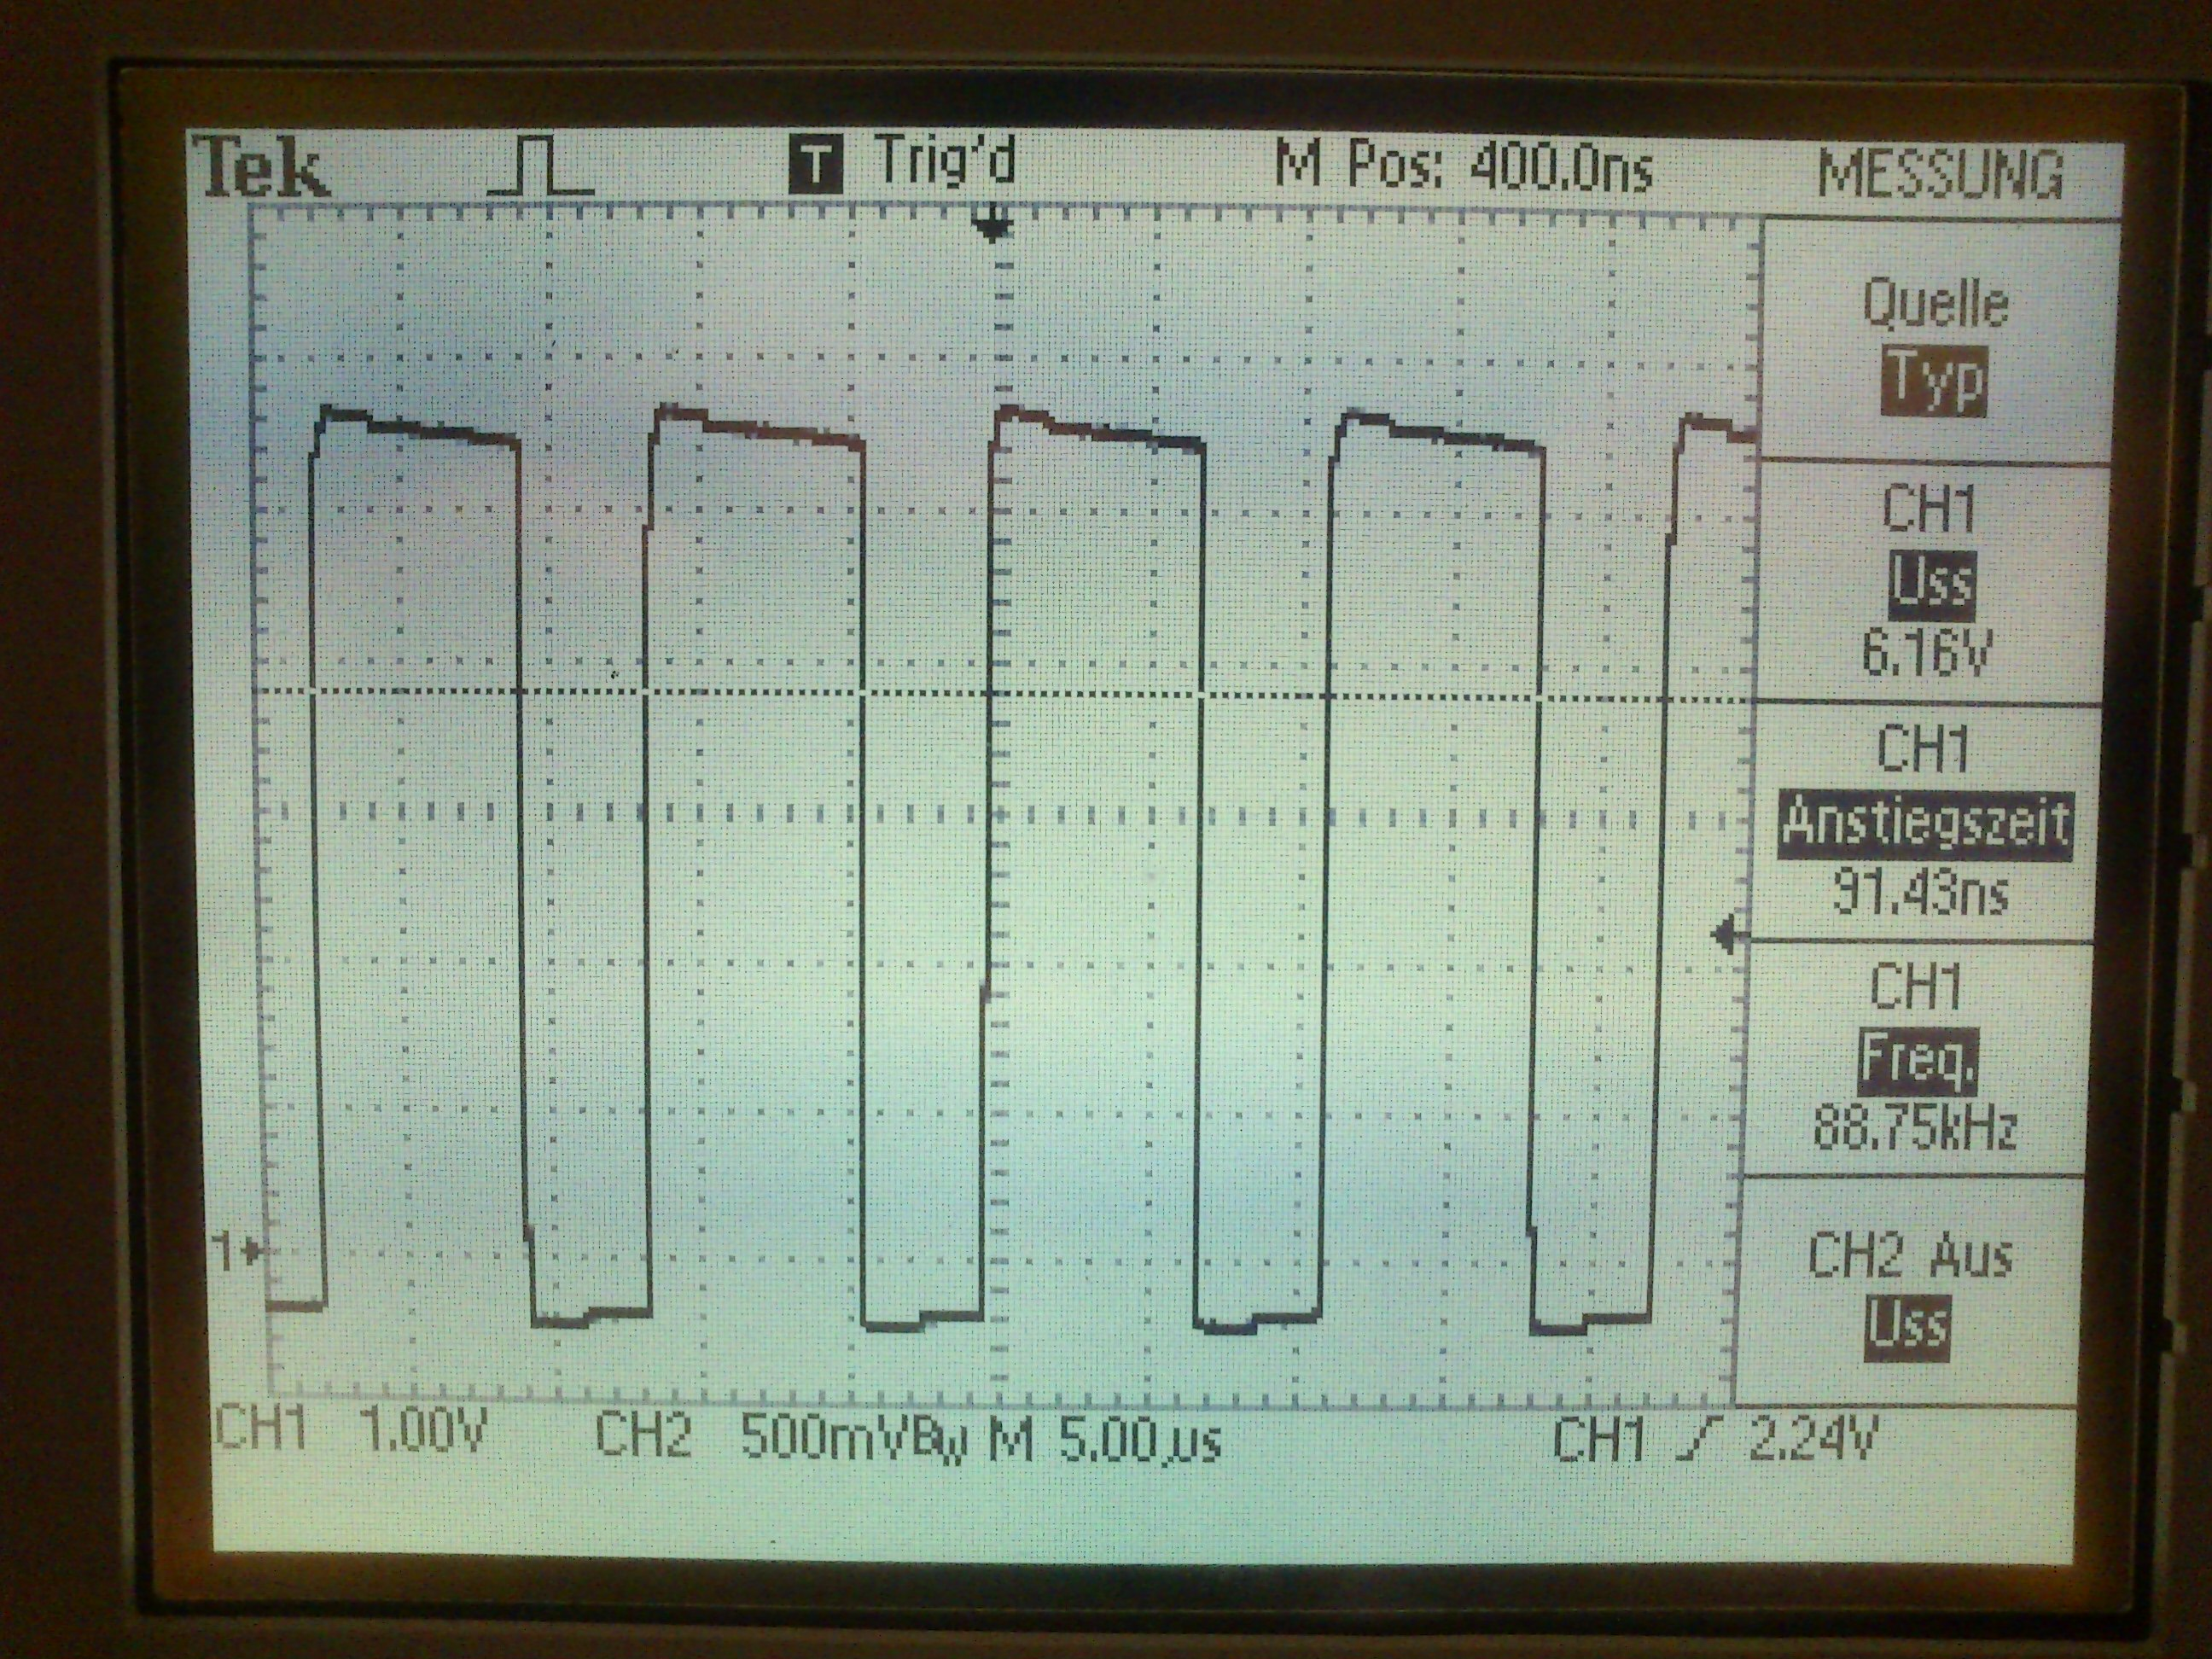
\includegraphics[width=\linewidth]{versuch3/oszi/DSC_0259.JPG}
	\caption{Frequenzmessung der Oszillatorfrequenz}
\end{figure}
Es zeigt sich deutlich das assymetrische Tastverhältnis. Es rührt von den verschiedenen Schaltschwellen des NE555 her, da er bei 1/3 $ U_{cc} $ des Kondensators gesetzt, aber bei 2/3 $ U_{cc} $ gelöscht wird.

Wenn man parallel einen weiteren 100µF-Kondensator verbaut, sinkt die Frequenz auf rund 5 Hz:
\begin{figure}[H]
	\centering
	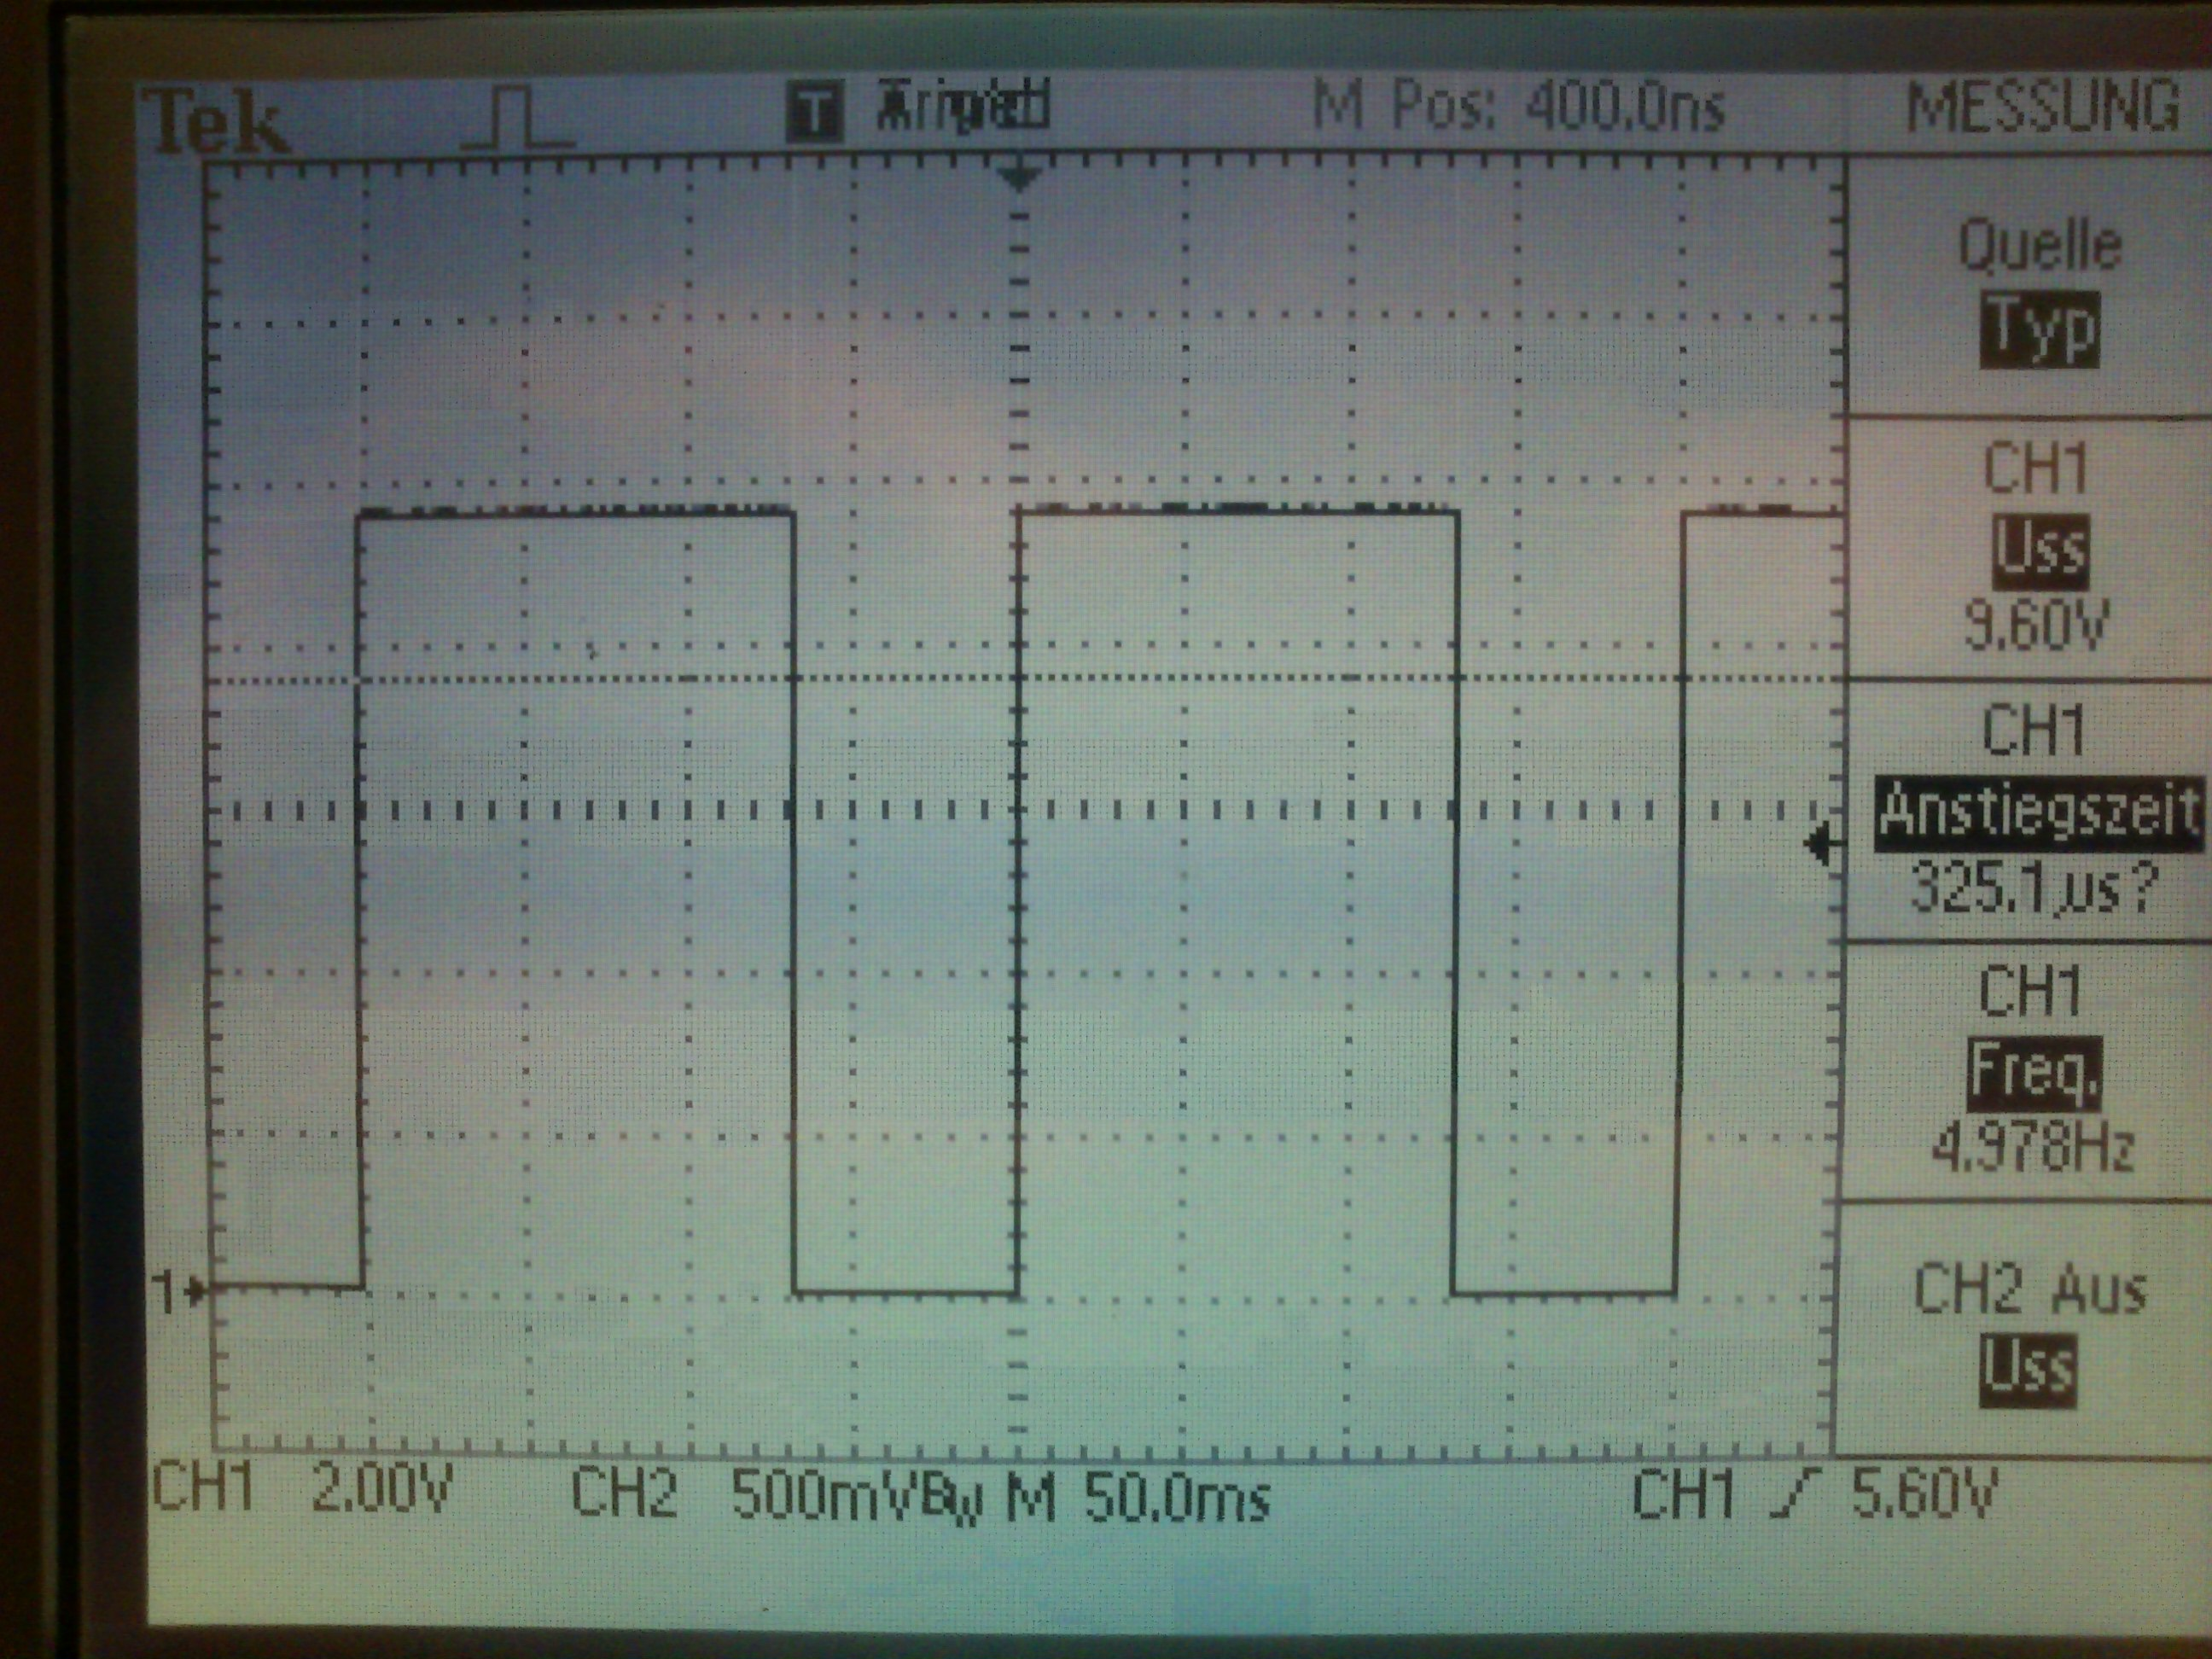
\includegraphics[width=\linewidth]{versuch3/oszi/DSC_0268.JPG}
	\caption{Frequenzmessung der Oszillatorfrequenz bei vergrößerter Kapazität}
\end{figure}
%}}}

%{{{
\subsection{Hoch- und Tiefpass}
In diesem Versuch wurde die Impulsantwort von Hochpass und Tiefpass bestimmt. Dazu wurde der im letzten Versuch aufgebaute Ozsillator wieder mit 5 Hz betrieben und das Filter auf den Ausgang gesteckt.
\begin{figure}
	\centering
	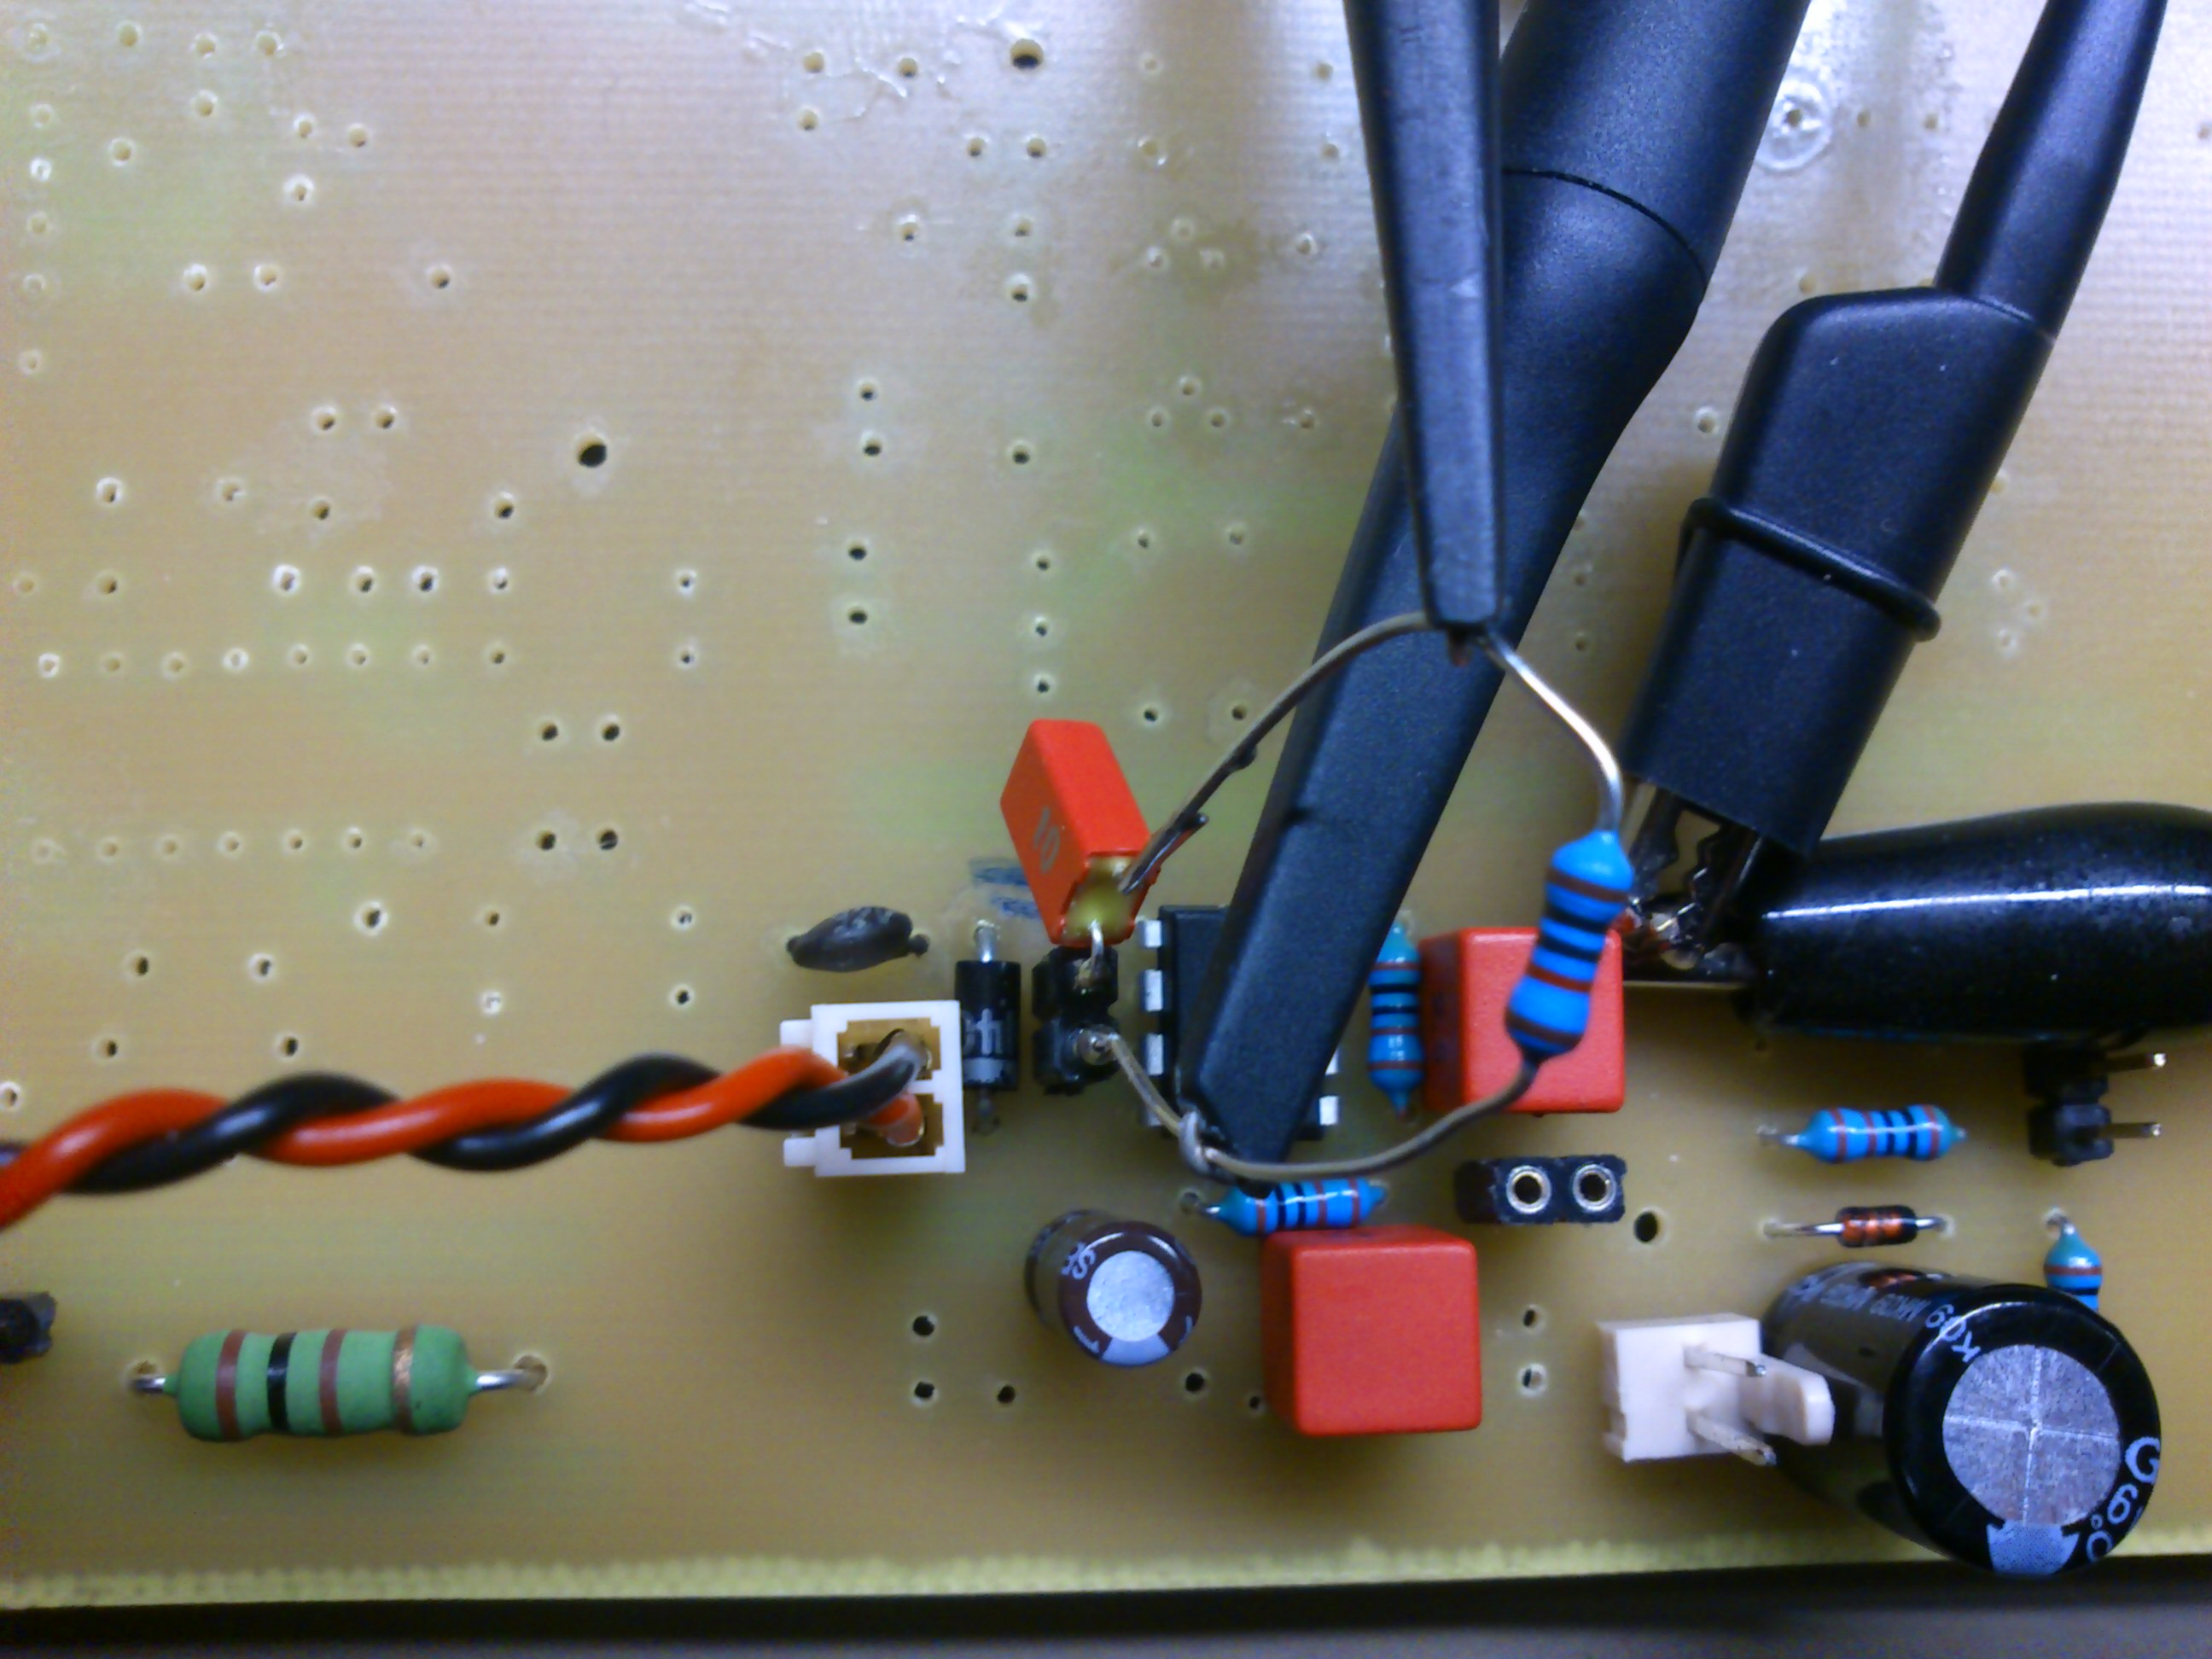
\includegraphics[width=\linewidth]{versuch3/oszi/DSC_0274.JPG}
	\caption{Das eingebaute Filter}
\end{figure}
Die Impulsantwort ergab sich wie folgt:
\begin{figure}[H]
	\centering
	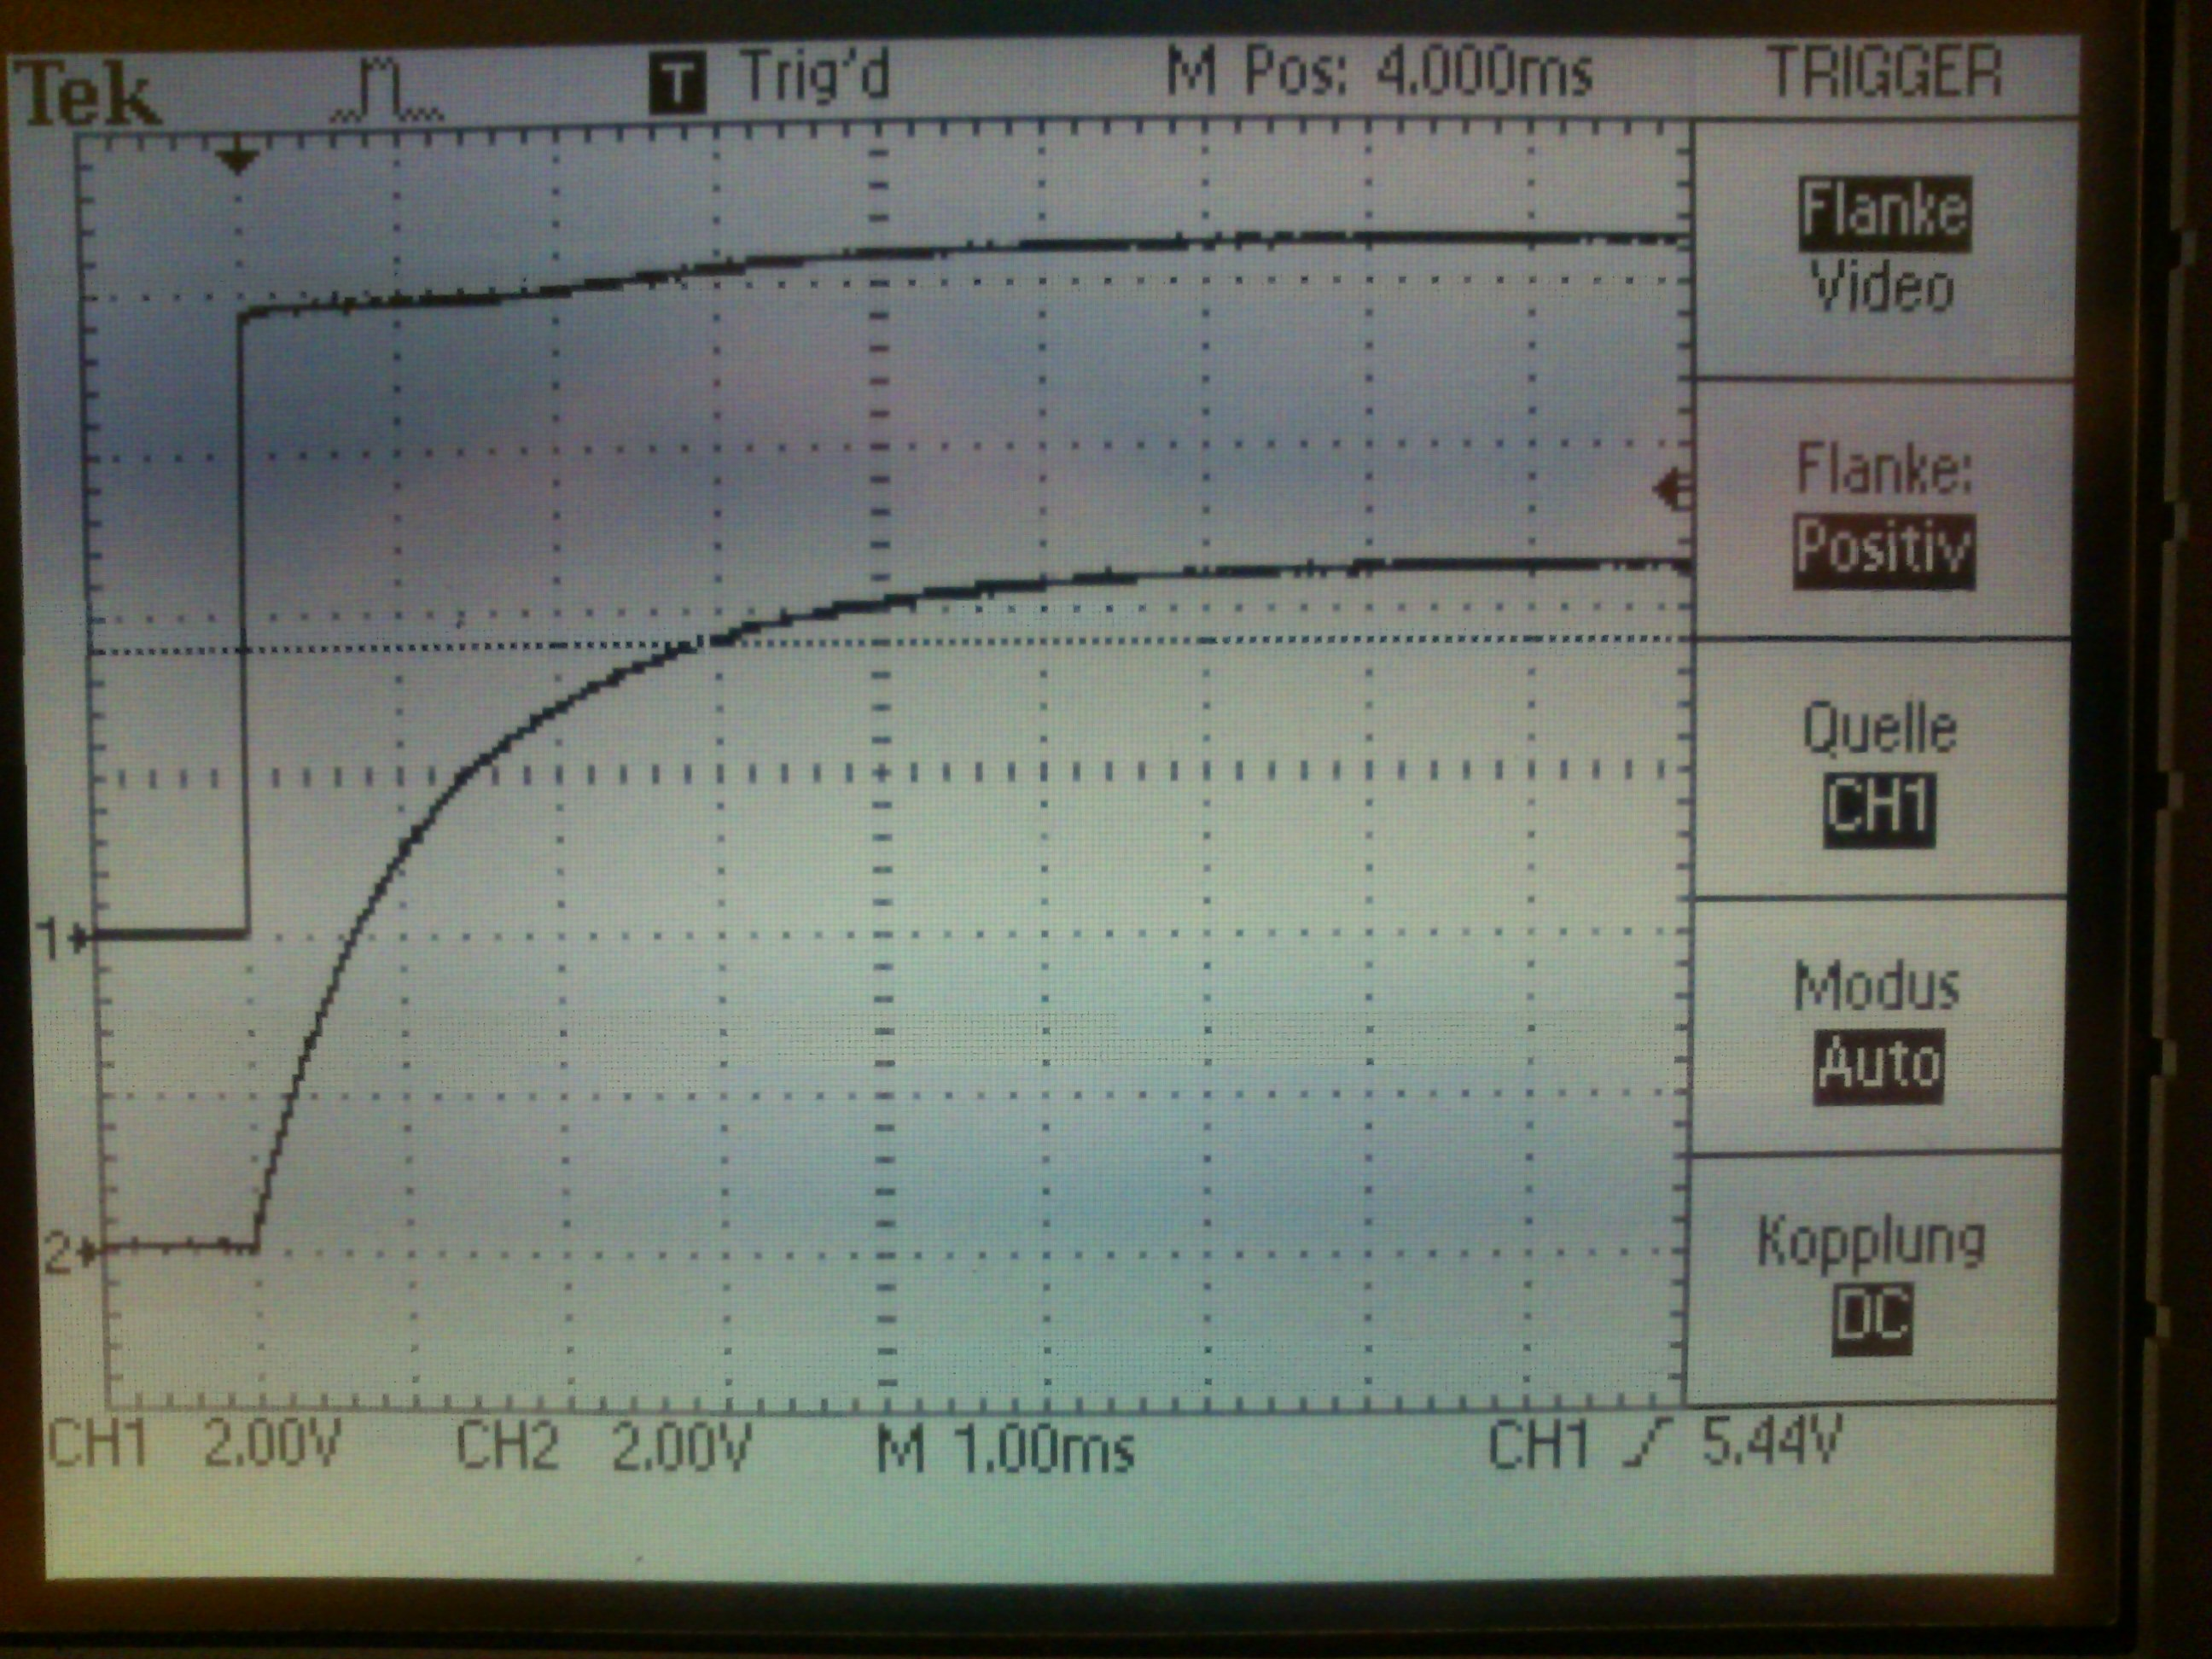
\includegraphics[width=\linewidth]{versuch3/oszi/DSC_0283.JPG}
	\caption{Impulsantwort des Tiefpasses}
\end{figure}

Dann wurde das Filter umgekehrt aufgesteckt, damit als Hochpass verwendet und dessen Impulsantwort bestimmt:
\begin{figure}[H]
	\centering
	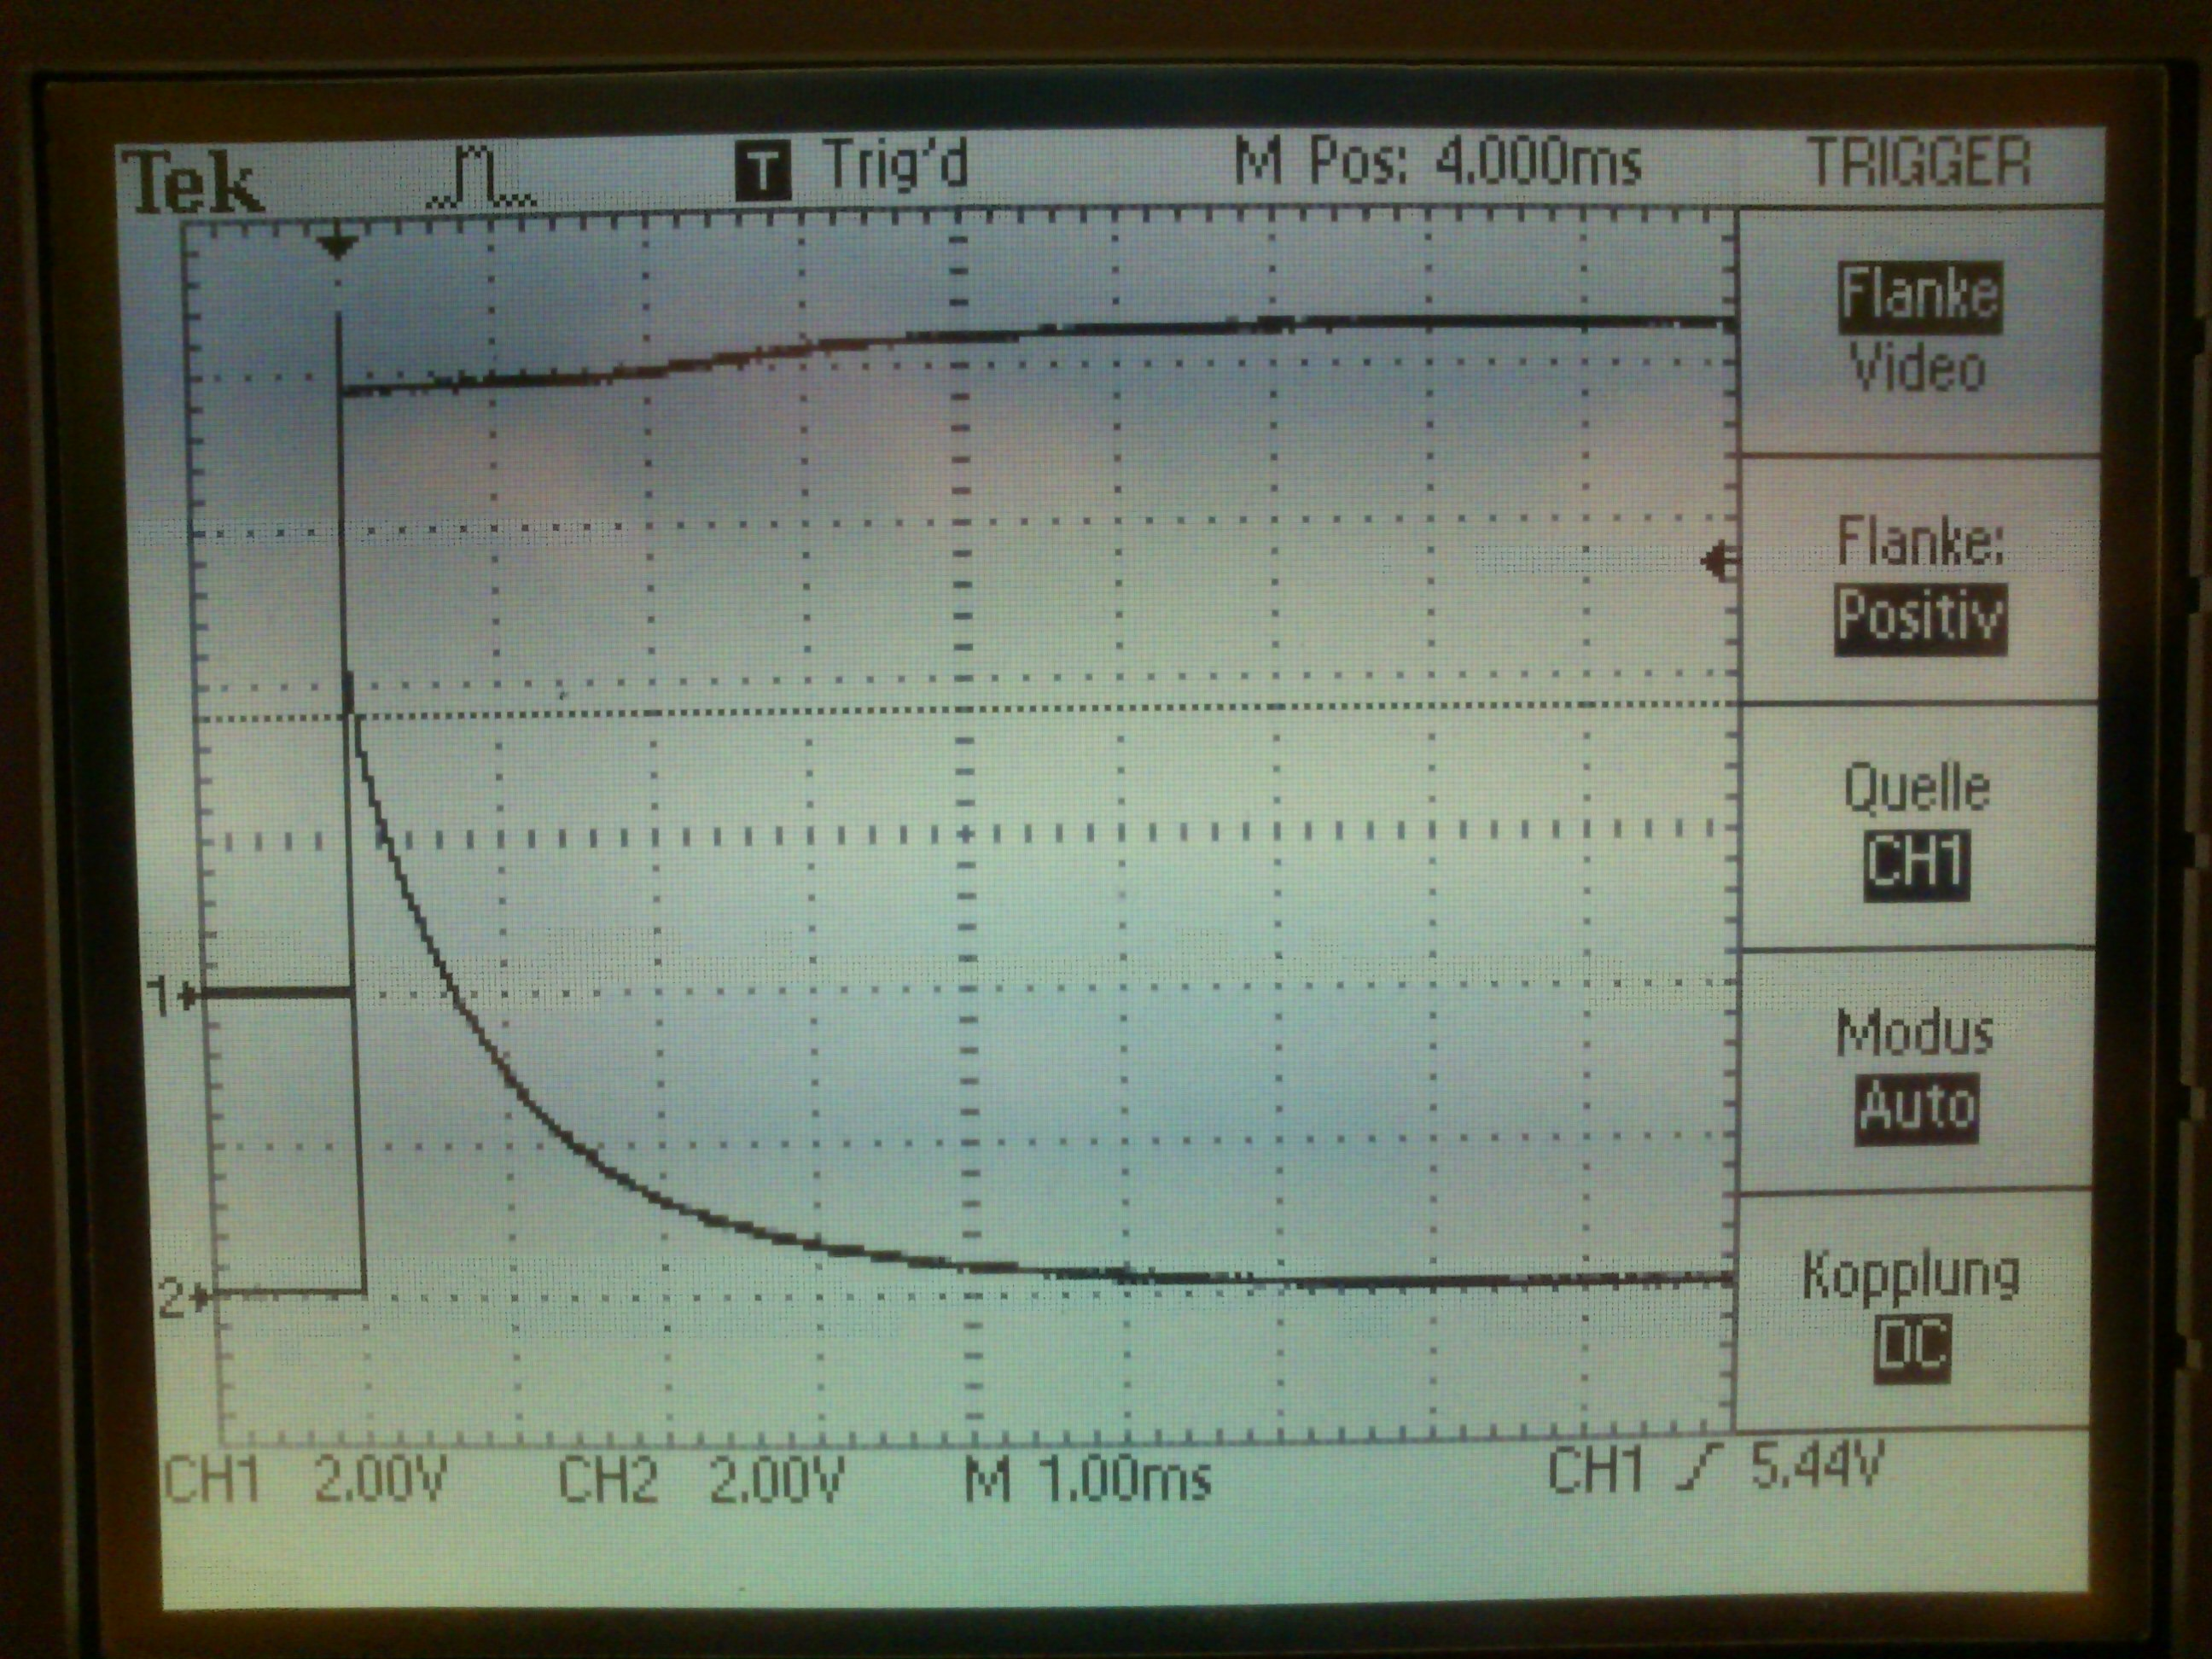
\includegraphics[width=\linewidth]{versuch3/oszi/DSC_0287.JPG}
	\caption{Impulsantwort des Hochpasses}
\end{figure}
%}}}

%{{{
\subsection{Untere Grenzfrequenz des Oszilloskop}
In diesem Versuch wurden 2 Methoden verwendet, um die untere Grenzfrequenz des Oszilloskops zu bestimmen.
\subsubsection*{Direkte Messung}
Hierzu wurde die Frequenz am Generator so lange herunter gedreht, bis die gemessene Spannung am Oszilloskop auf $\sqrt{2}$ mal die Versorgungsspannung abgesunken war:

\begin{figure}[H]
	\begin{minipage}[b]{0.5\linewidth}
		\centering
		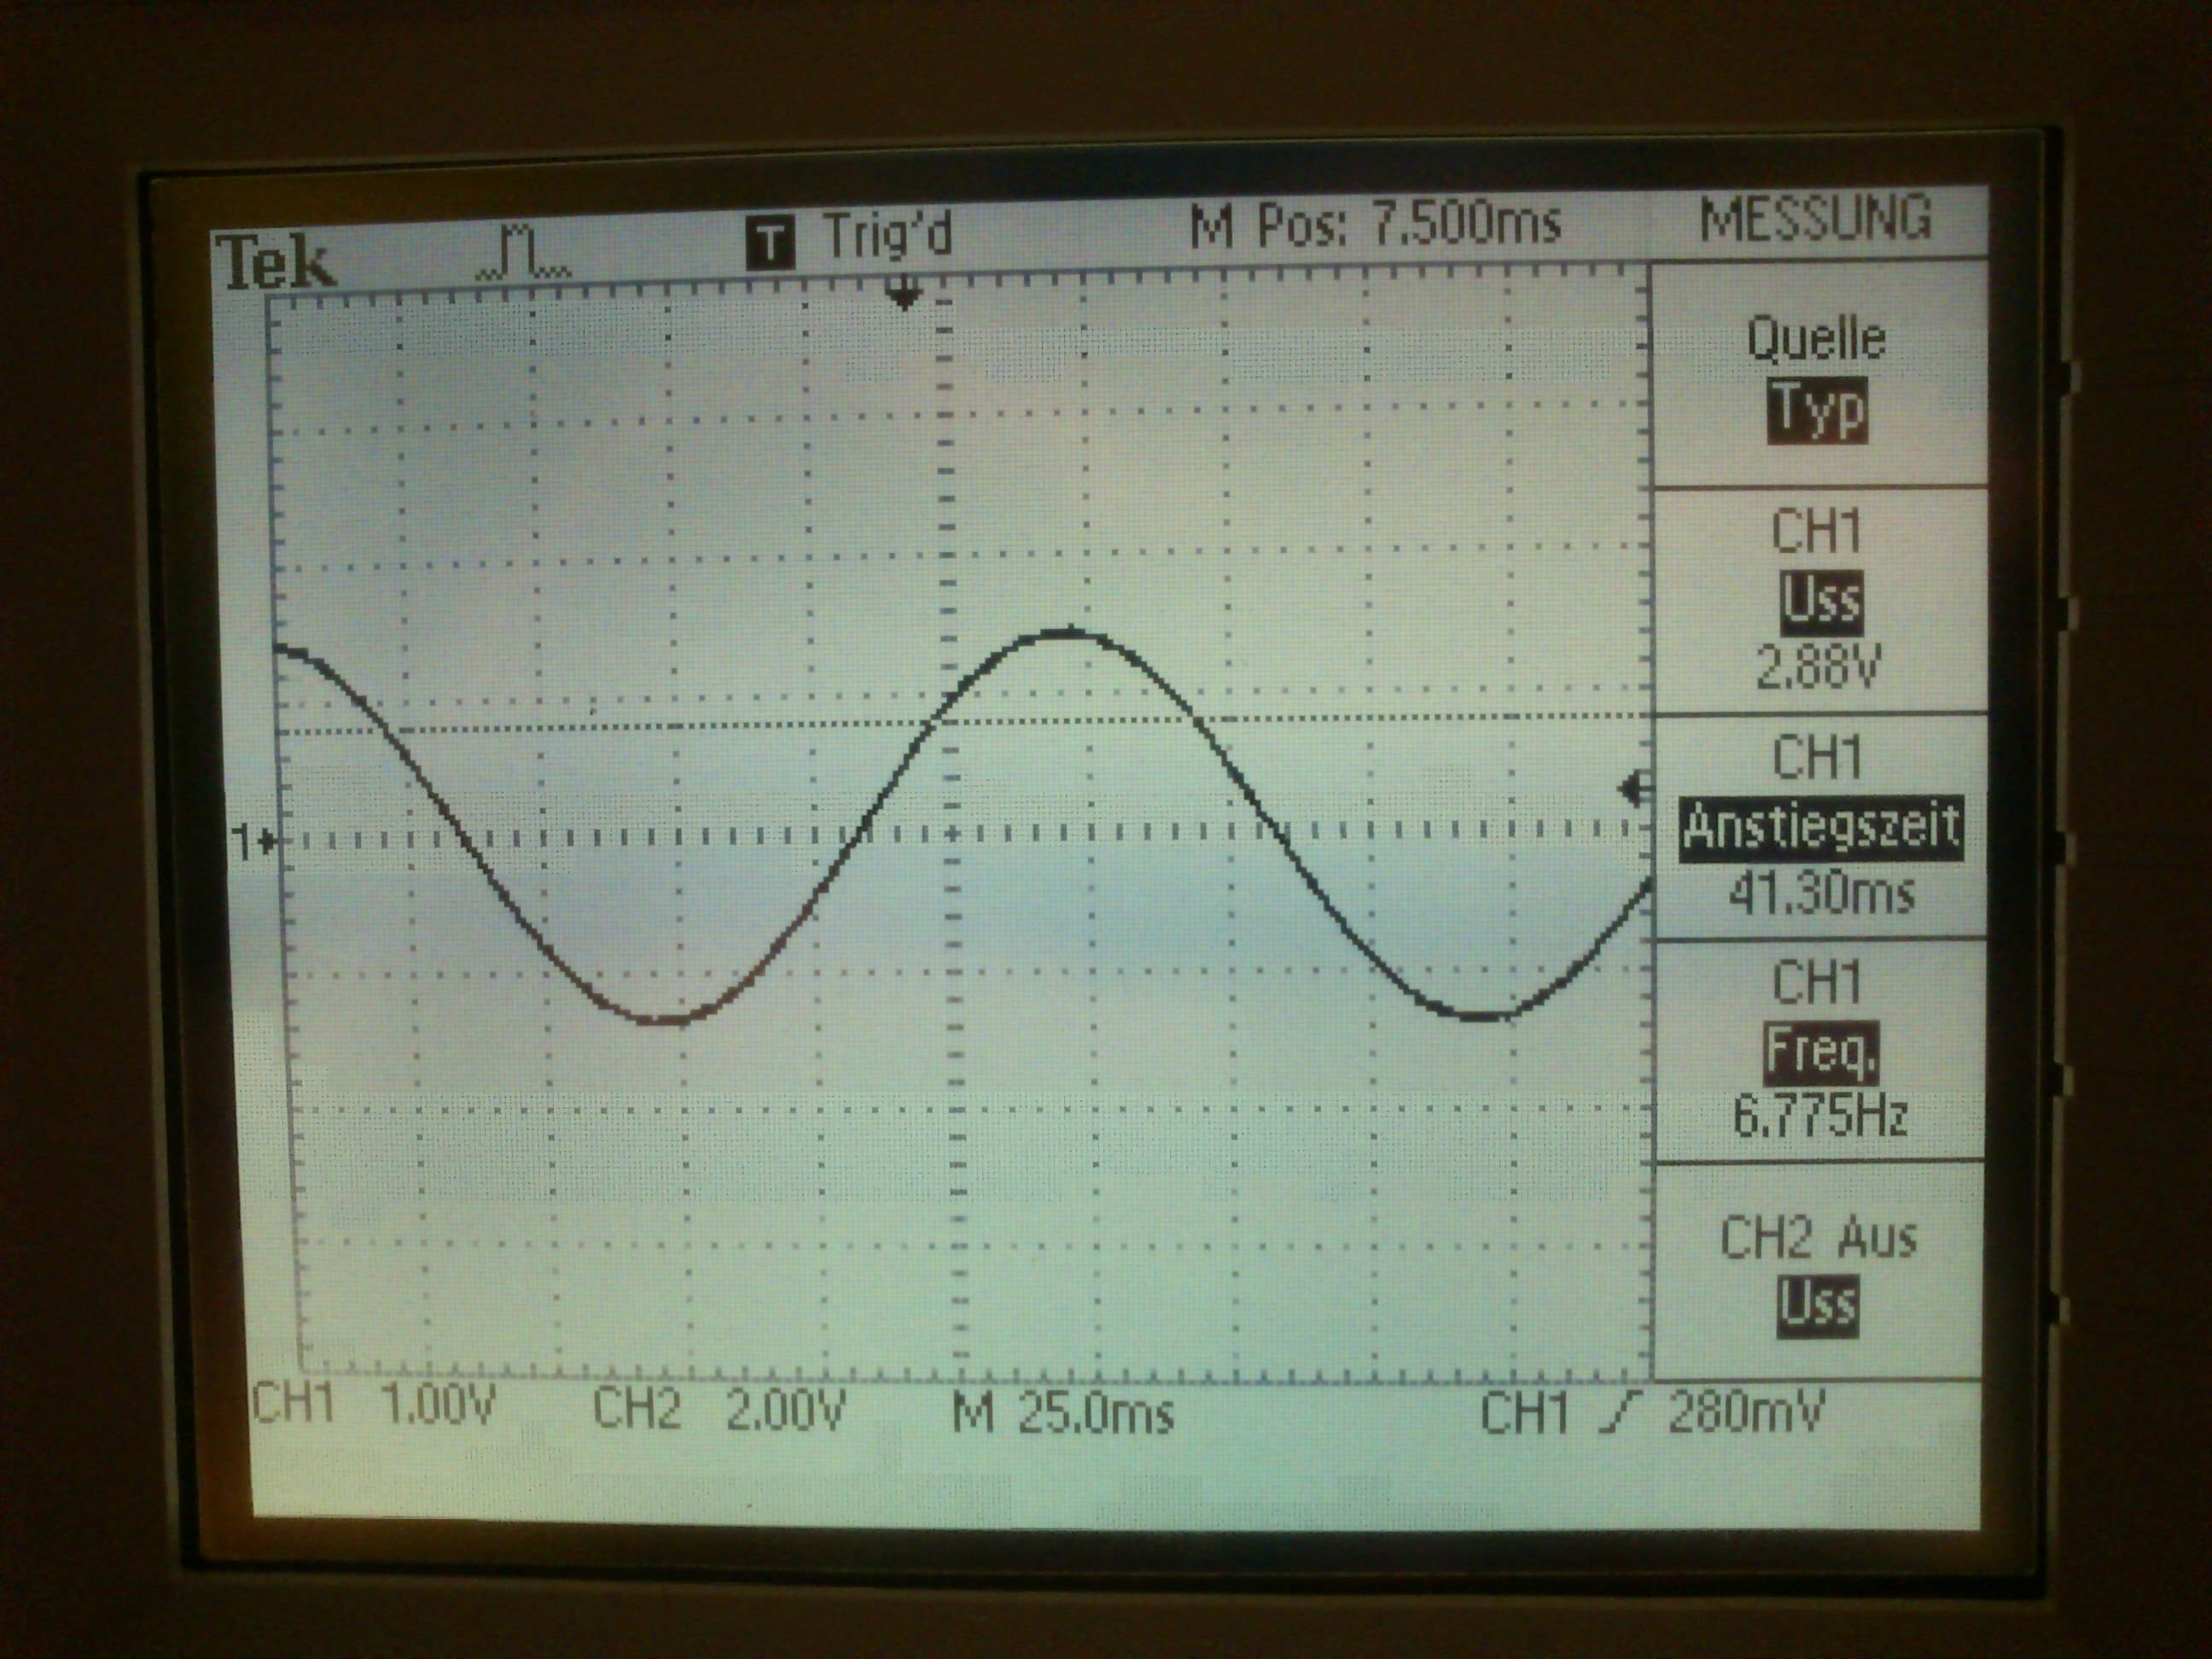
\includegraphics[width=\linewidth]{versuch3/oszi/DSC_0295.JPG}
		\caption{Ermittlung der Spannung \ldots}
	\end{minipage}
	\hspace{0.5cm}
	\begin{minipage}[b]{0.5\linewidth}
		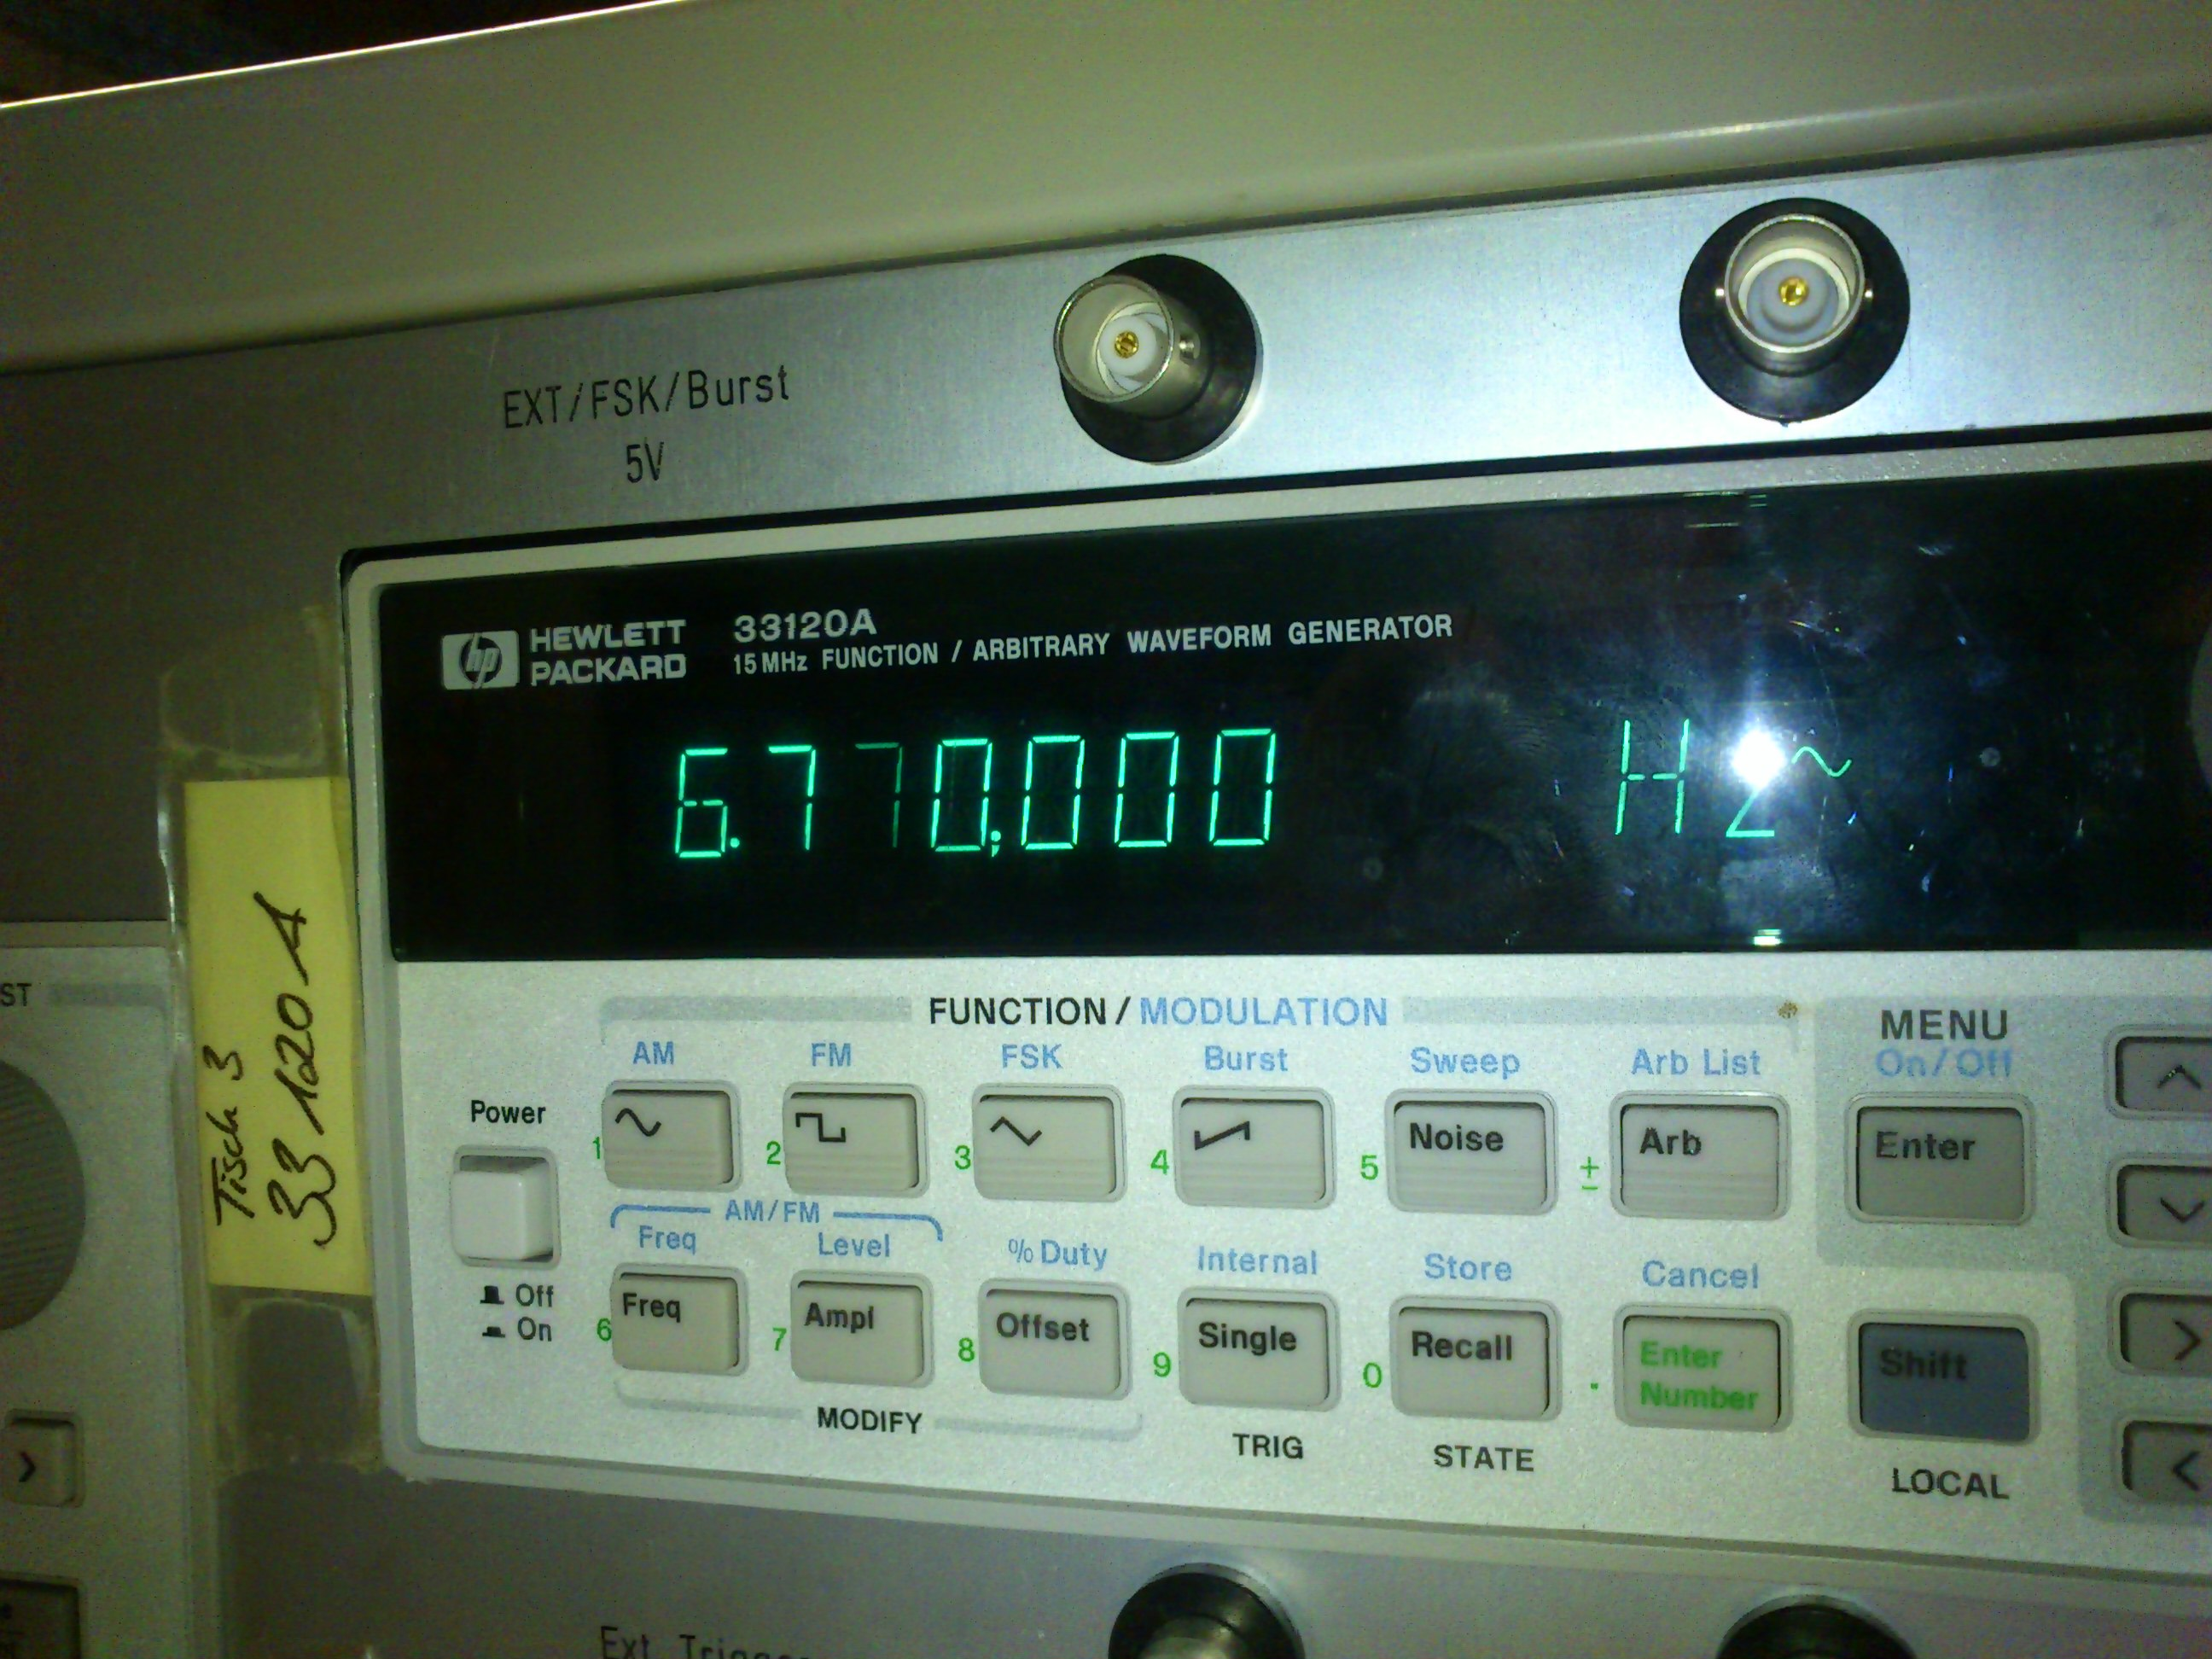
\includegraphics[width=\linewidth]{versuch3/oszi/DSC_0294.JPG}
		\caption{\ldots und die Grenzfrequenz}
		\centering
	\end{minipage}
\end{figure}
Somit ist der untere Grenzwert bei 6.77 Hz.

\subsubsection*{Dachschräge}
Bei dieser Möglichkeit wird die Dachschräge einer Rechteckspannung für die Messung der unteren Grenzfrequenz herangezogen:
\begin{figure}[H]
	\centering
	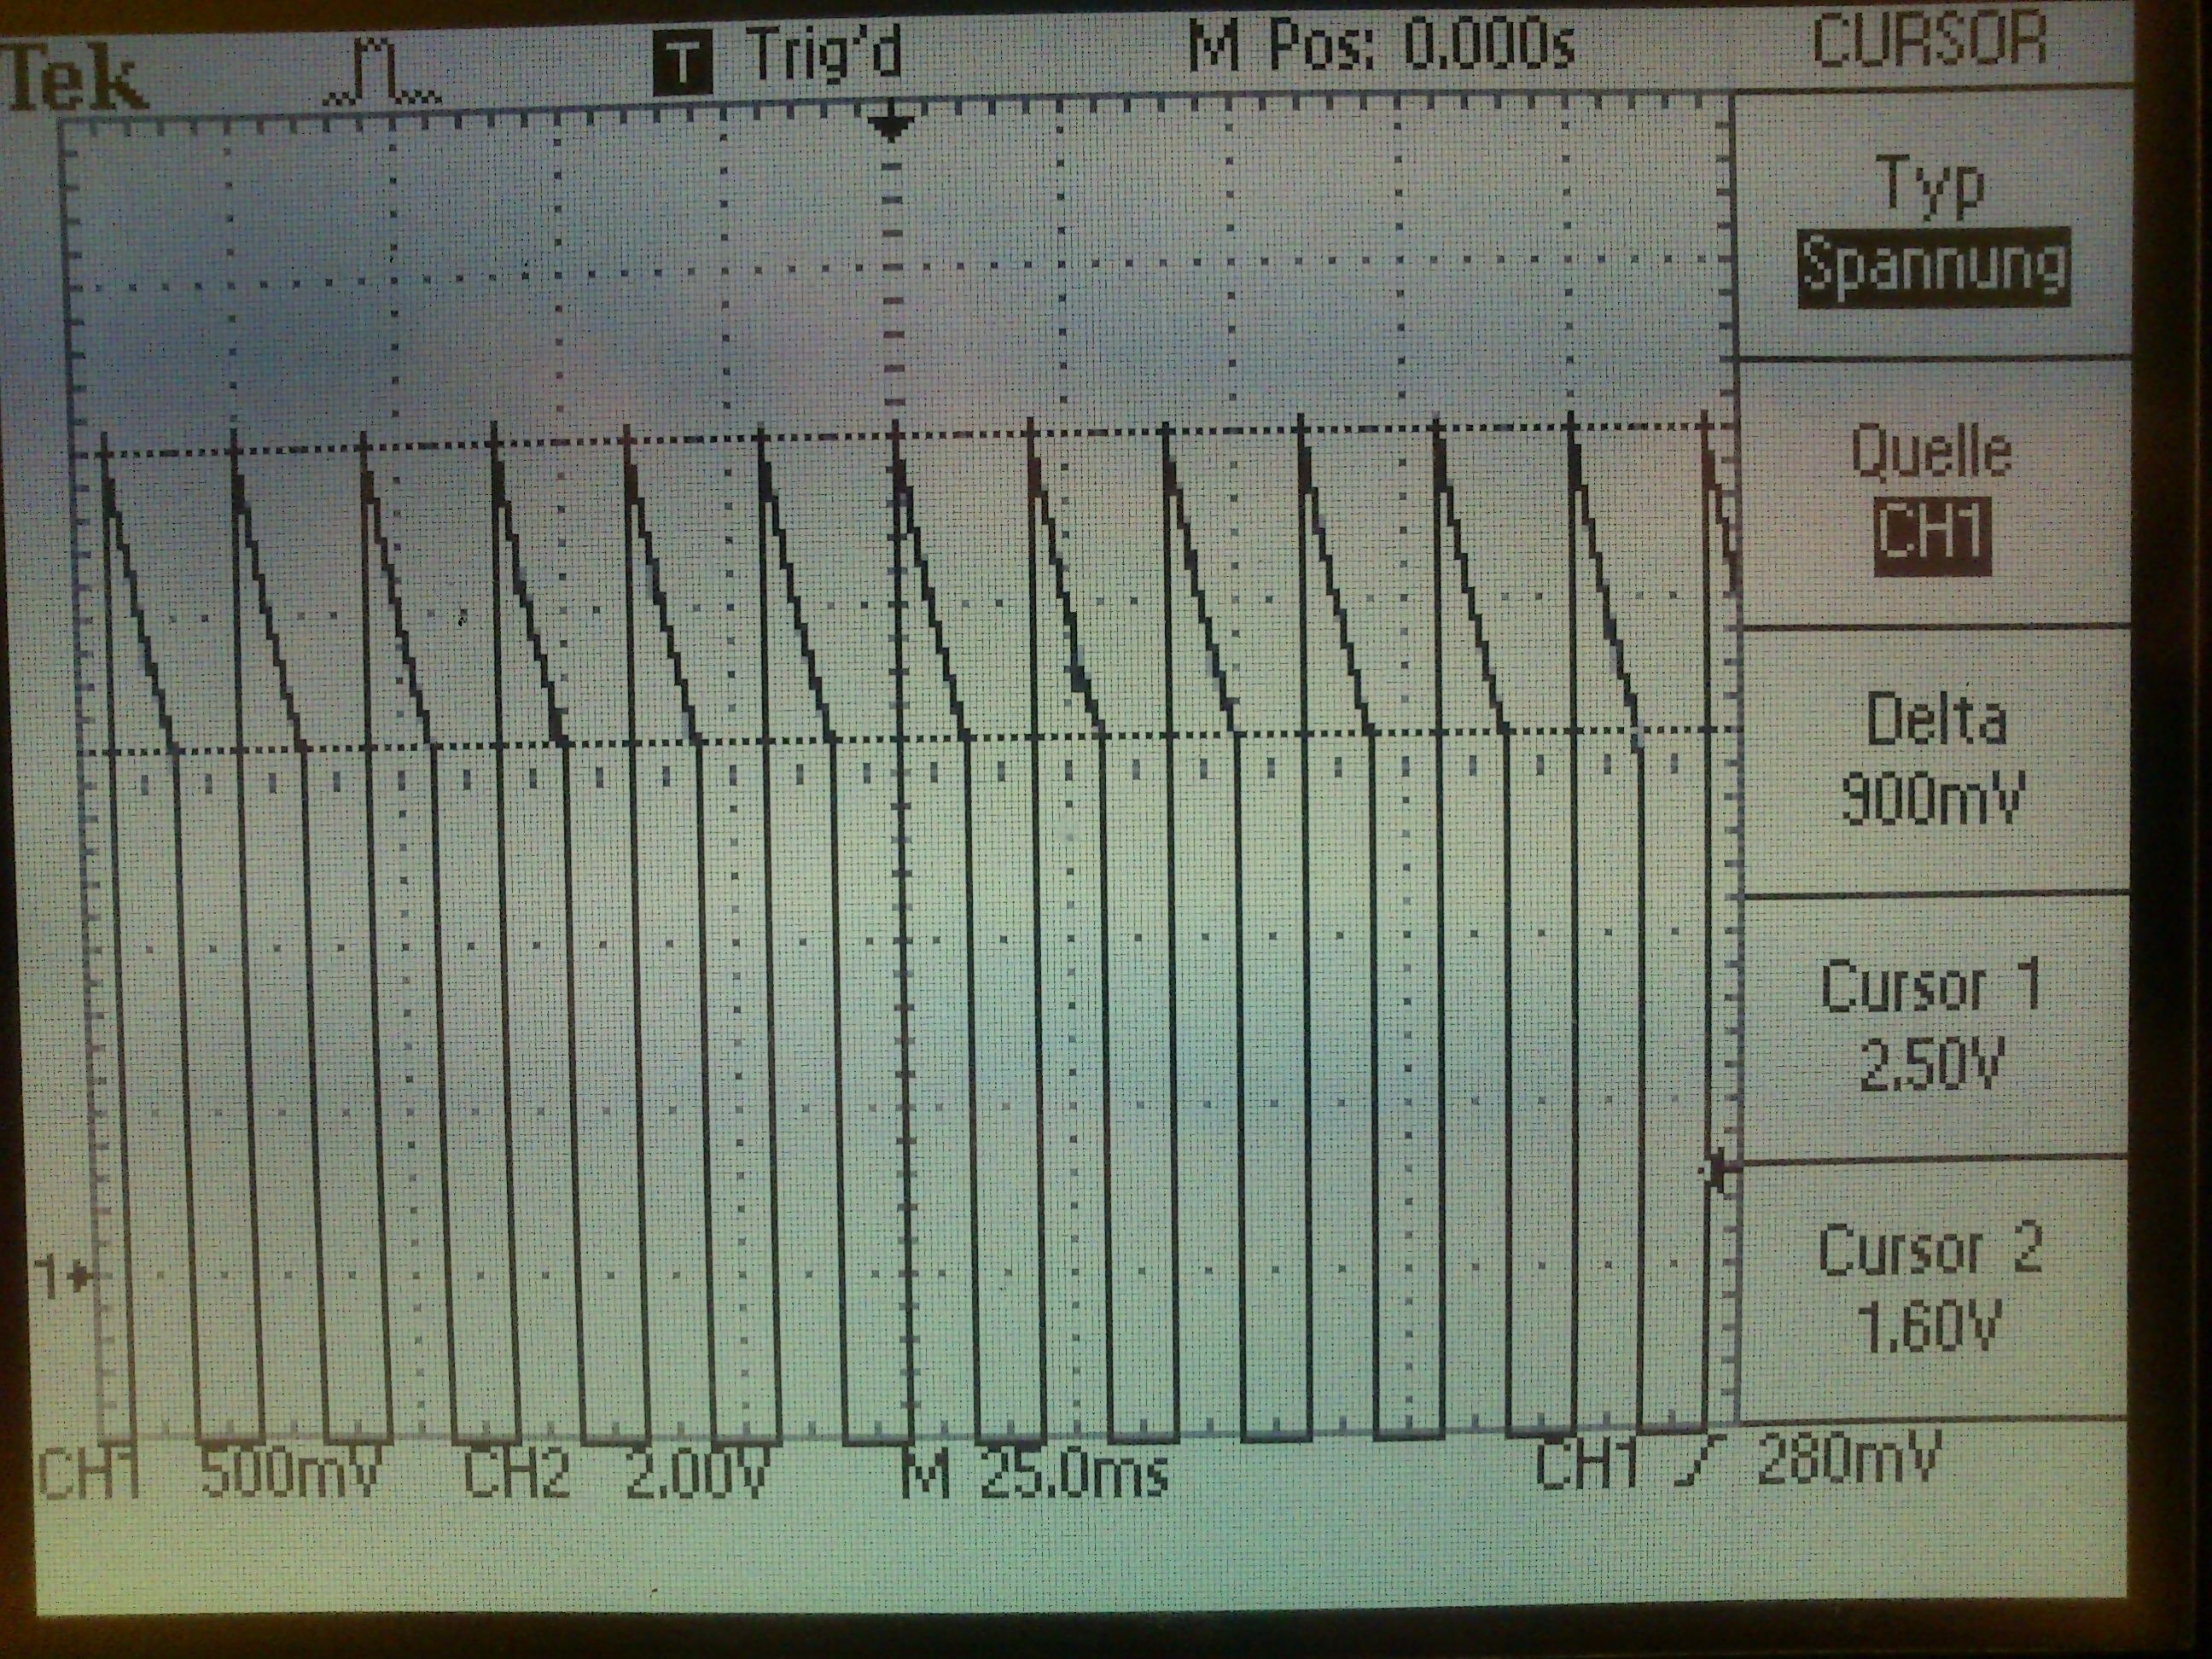
\includegraphics[width=\linewidth]{versuch3/oszi/DSC_0300.JPG}
	\caption{Dachschrägenmessung an einer 50Hz-Rechteckspannung: \Delta U}
\end{figure}
\begin{figure}[H]
	\centering
	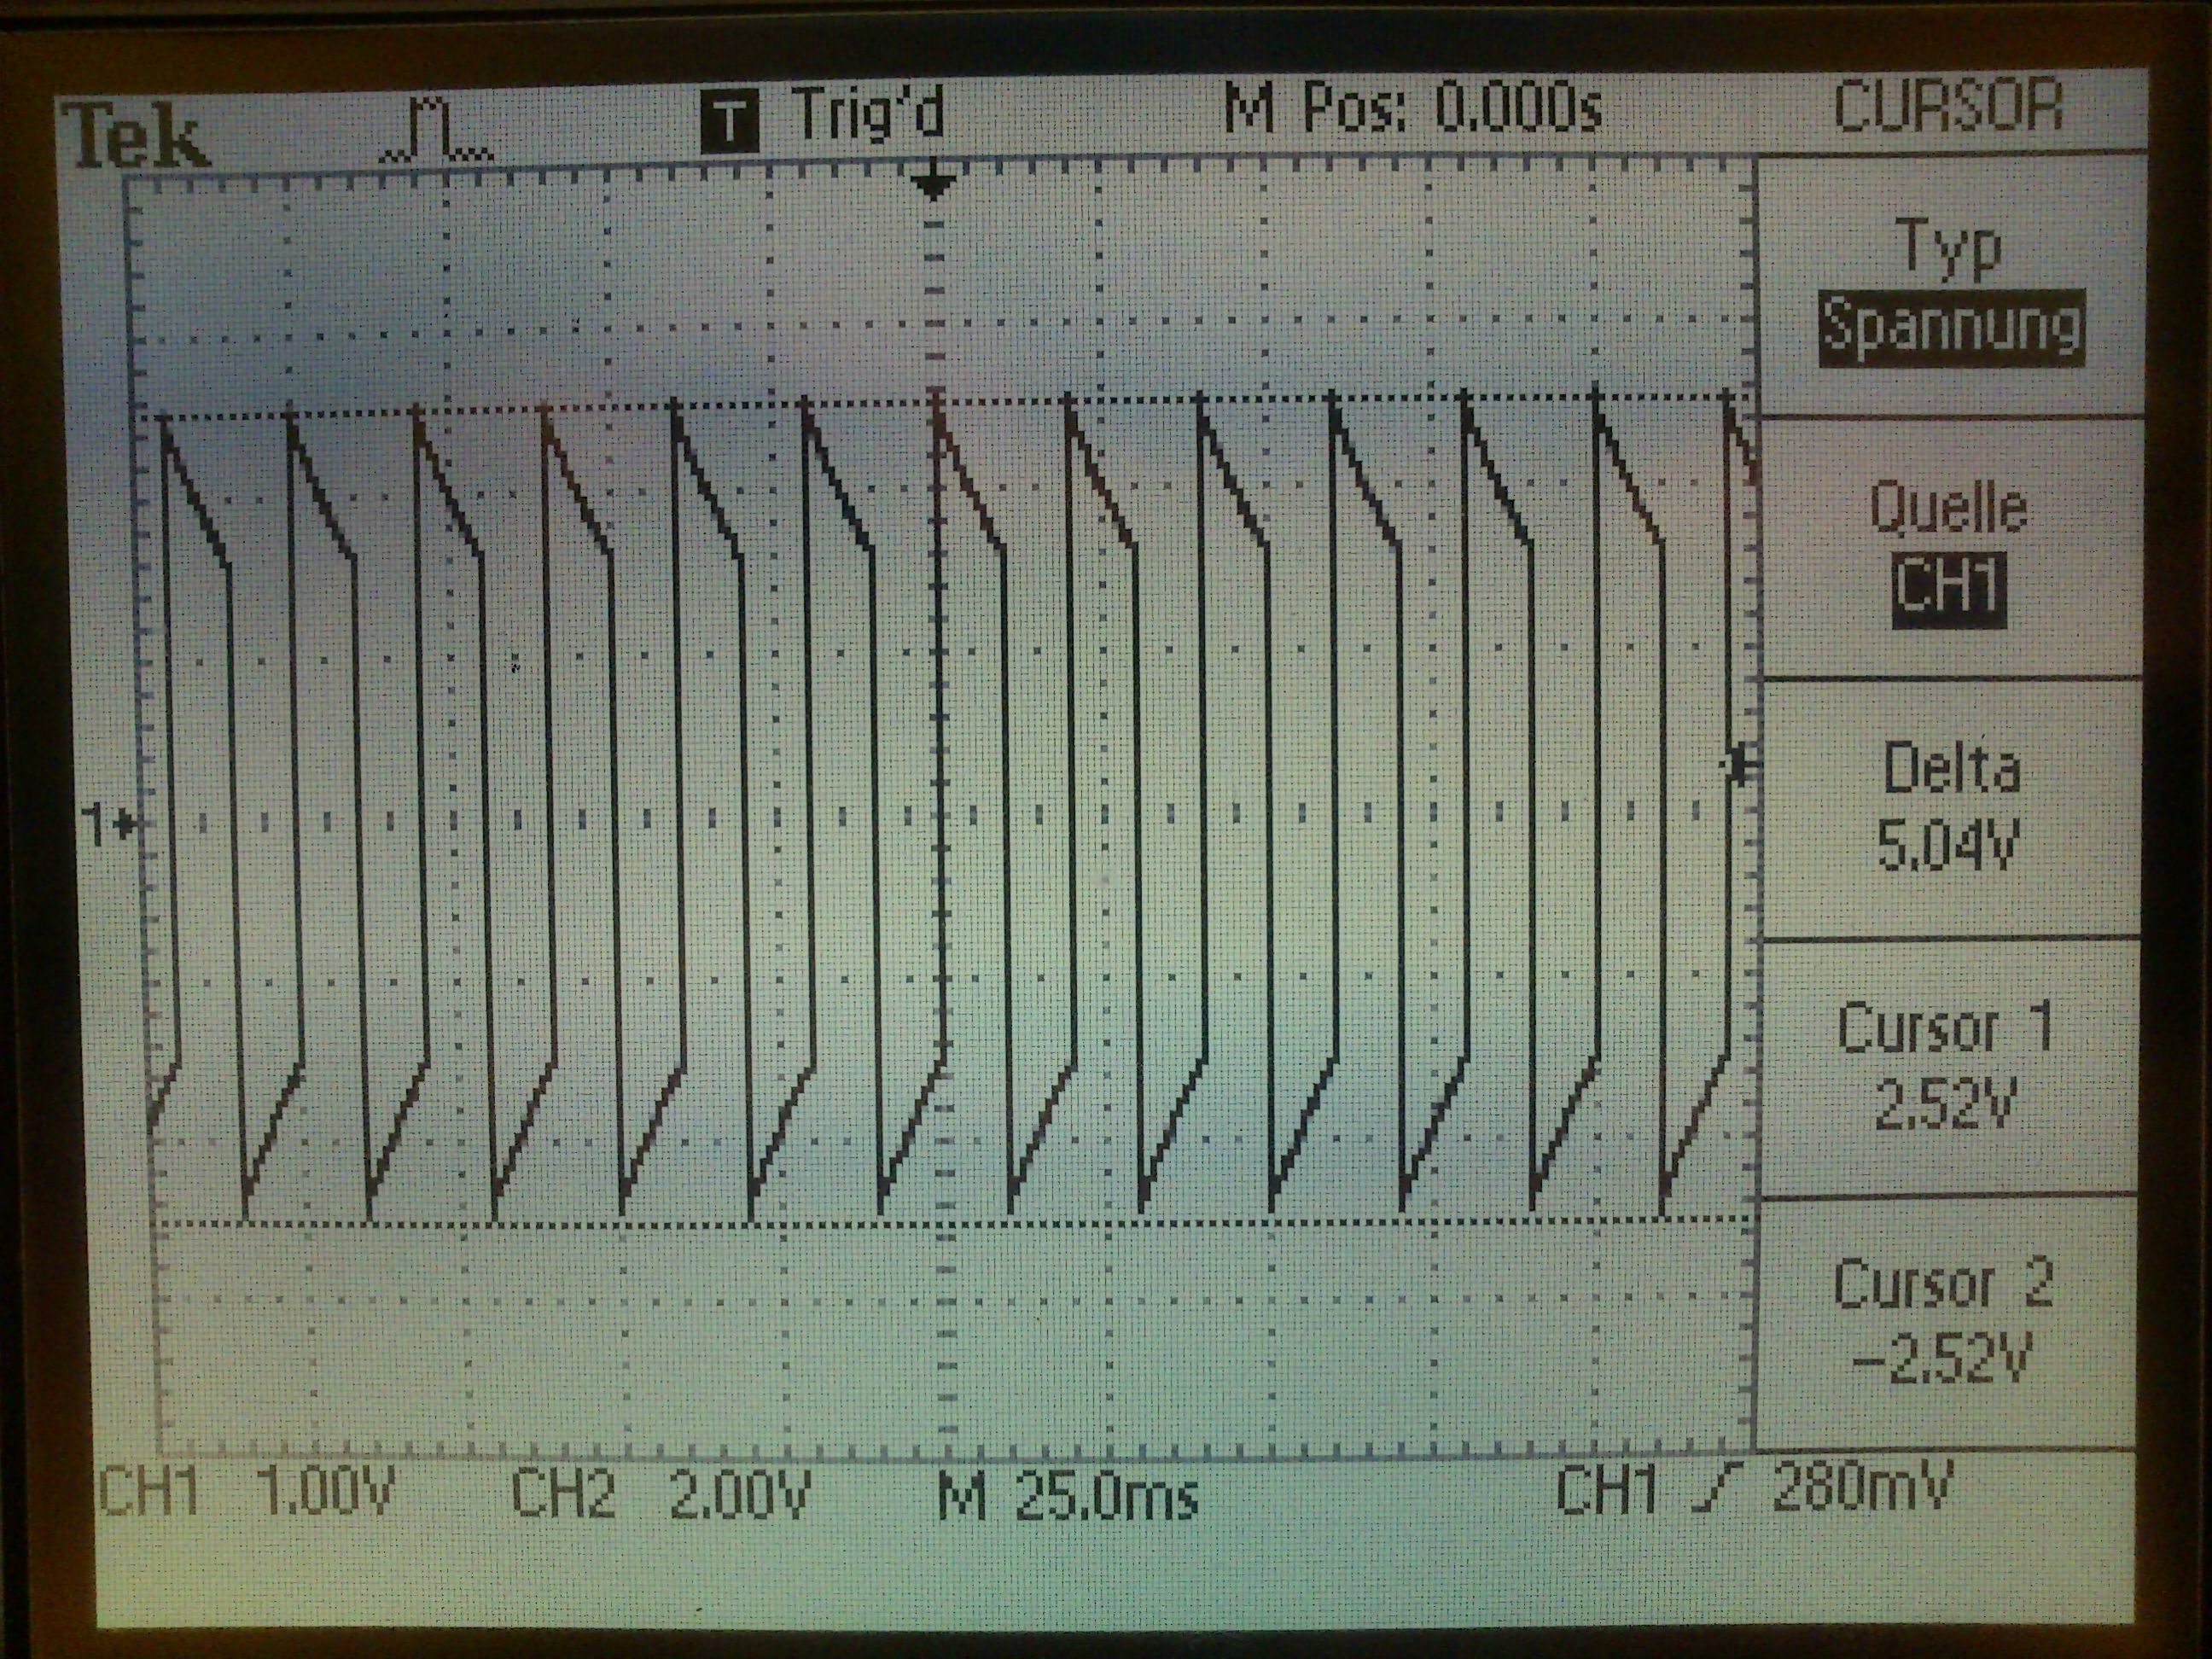
\includegraphics[width=\linewidth]{versuch3/oszi/DSC_0304.JPG}
	\caption{Dachschrägenmessung an einer 50Hz-Rechteckspannung: U\textsubscript{ss}}
\end{figure}
Damit lässt sich die untere Grenzfrequenz wie folgt berechnen:\\
$ D = 2 * ∆U/U_{ss}=0.9V/5.04V;\; f=50Hz $ \\
$ \Rightarrow f_{gu}=\frac{f}{\pi} * ln \frac{1}{1 – D} = \frac{50Hz}{\pi}*ln\frac{1}{1-D} = 3.1307 Hz $
Dieser Wert ist etwa halb so groß wie der mit Möglichkeit 1 gemessene Wert. Ich vermute, dass die erste Methode günstiger ist, weil sich die Scheitelspannung eines Sinuses besser ablesen lässt, und die Grenzfrequenz direkt am Signalgenerator abgelesen werden kann.
%}}}

%{{{
\subsection{Obere Grenzfrequenz und Bandbreite eines Rechtecksignals}
\subsubsection*{Grenzfrequenz}
\begin{figure}[H]
	\centering
	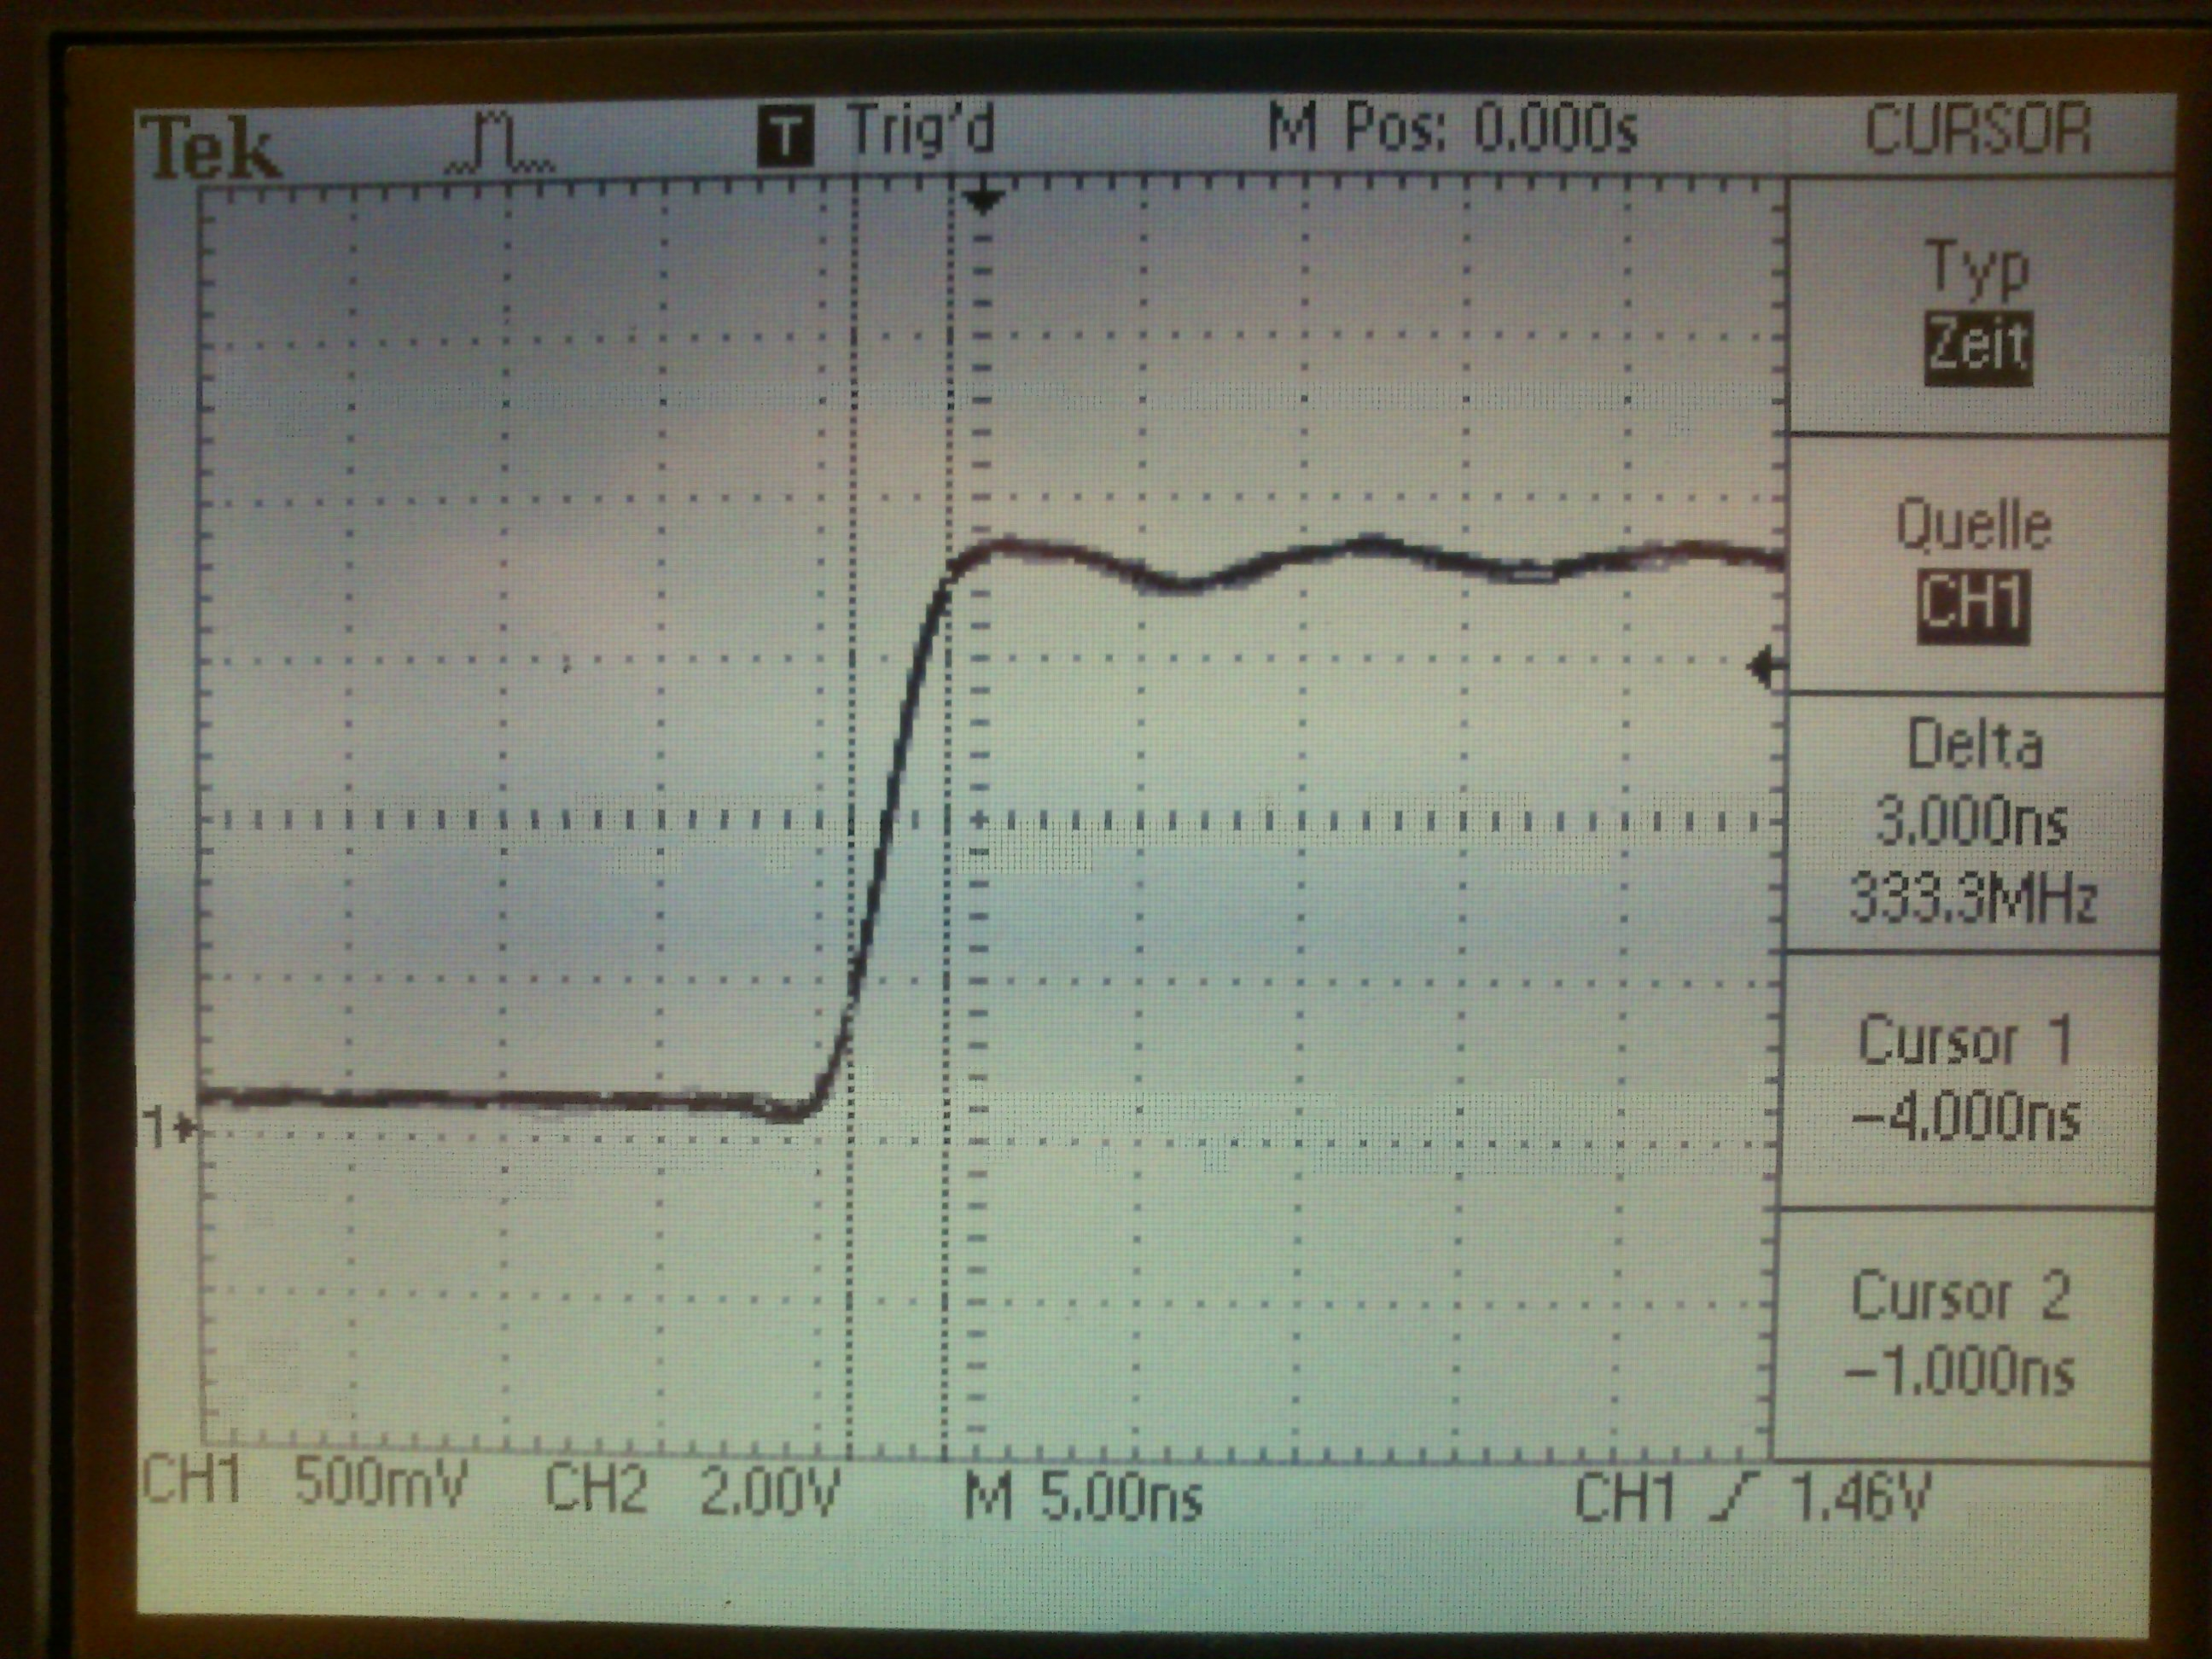
\includegraphics[width=\linewidth]{versuch3/oszi/DSC_0313.JPG}
	\caption{Messung der Anstiegszeit T\textsubscript{ges} am Sync-Ausgang}
\end{figure}
Da weiterhin bekannt ist, dass die Eigenanstiegszeit (t\textsubscript{sync}) des Signalgenerators 1,4 ns beträgt, kann man die obere Grenzfrequenz berechnen:\\
$ t_oszi = \sqrt{t_ges^2 - t_sync^2} = 2.6533 ns; \; \Rightarrow f_{og} = 0.35/t_oszi = 1.3191*10^8 Hz = 131.91 MHz $
Somit ist die berechnete Frequenz etwa 1,3 mal so groß, wie die Geräteangabe.
\subsubsection*{Anstiegszeit der Rechteckspannung}
\begin{figure}[H]
	\centering
	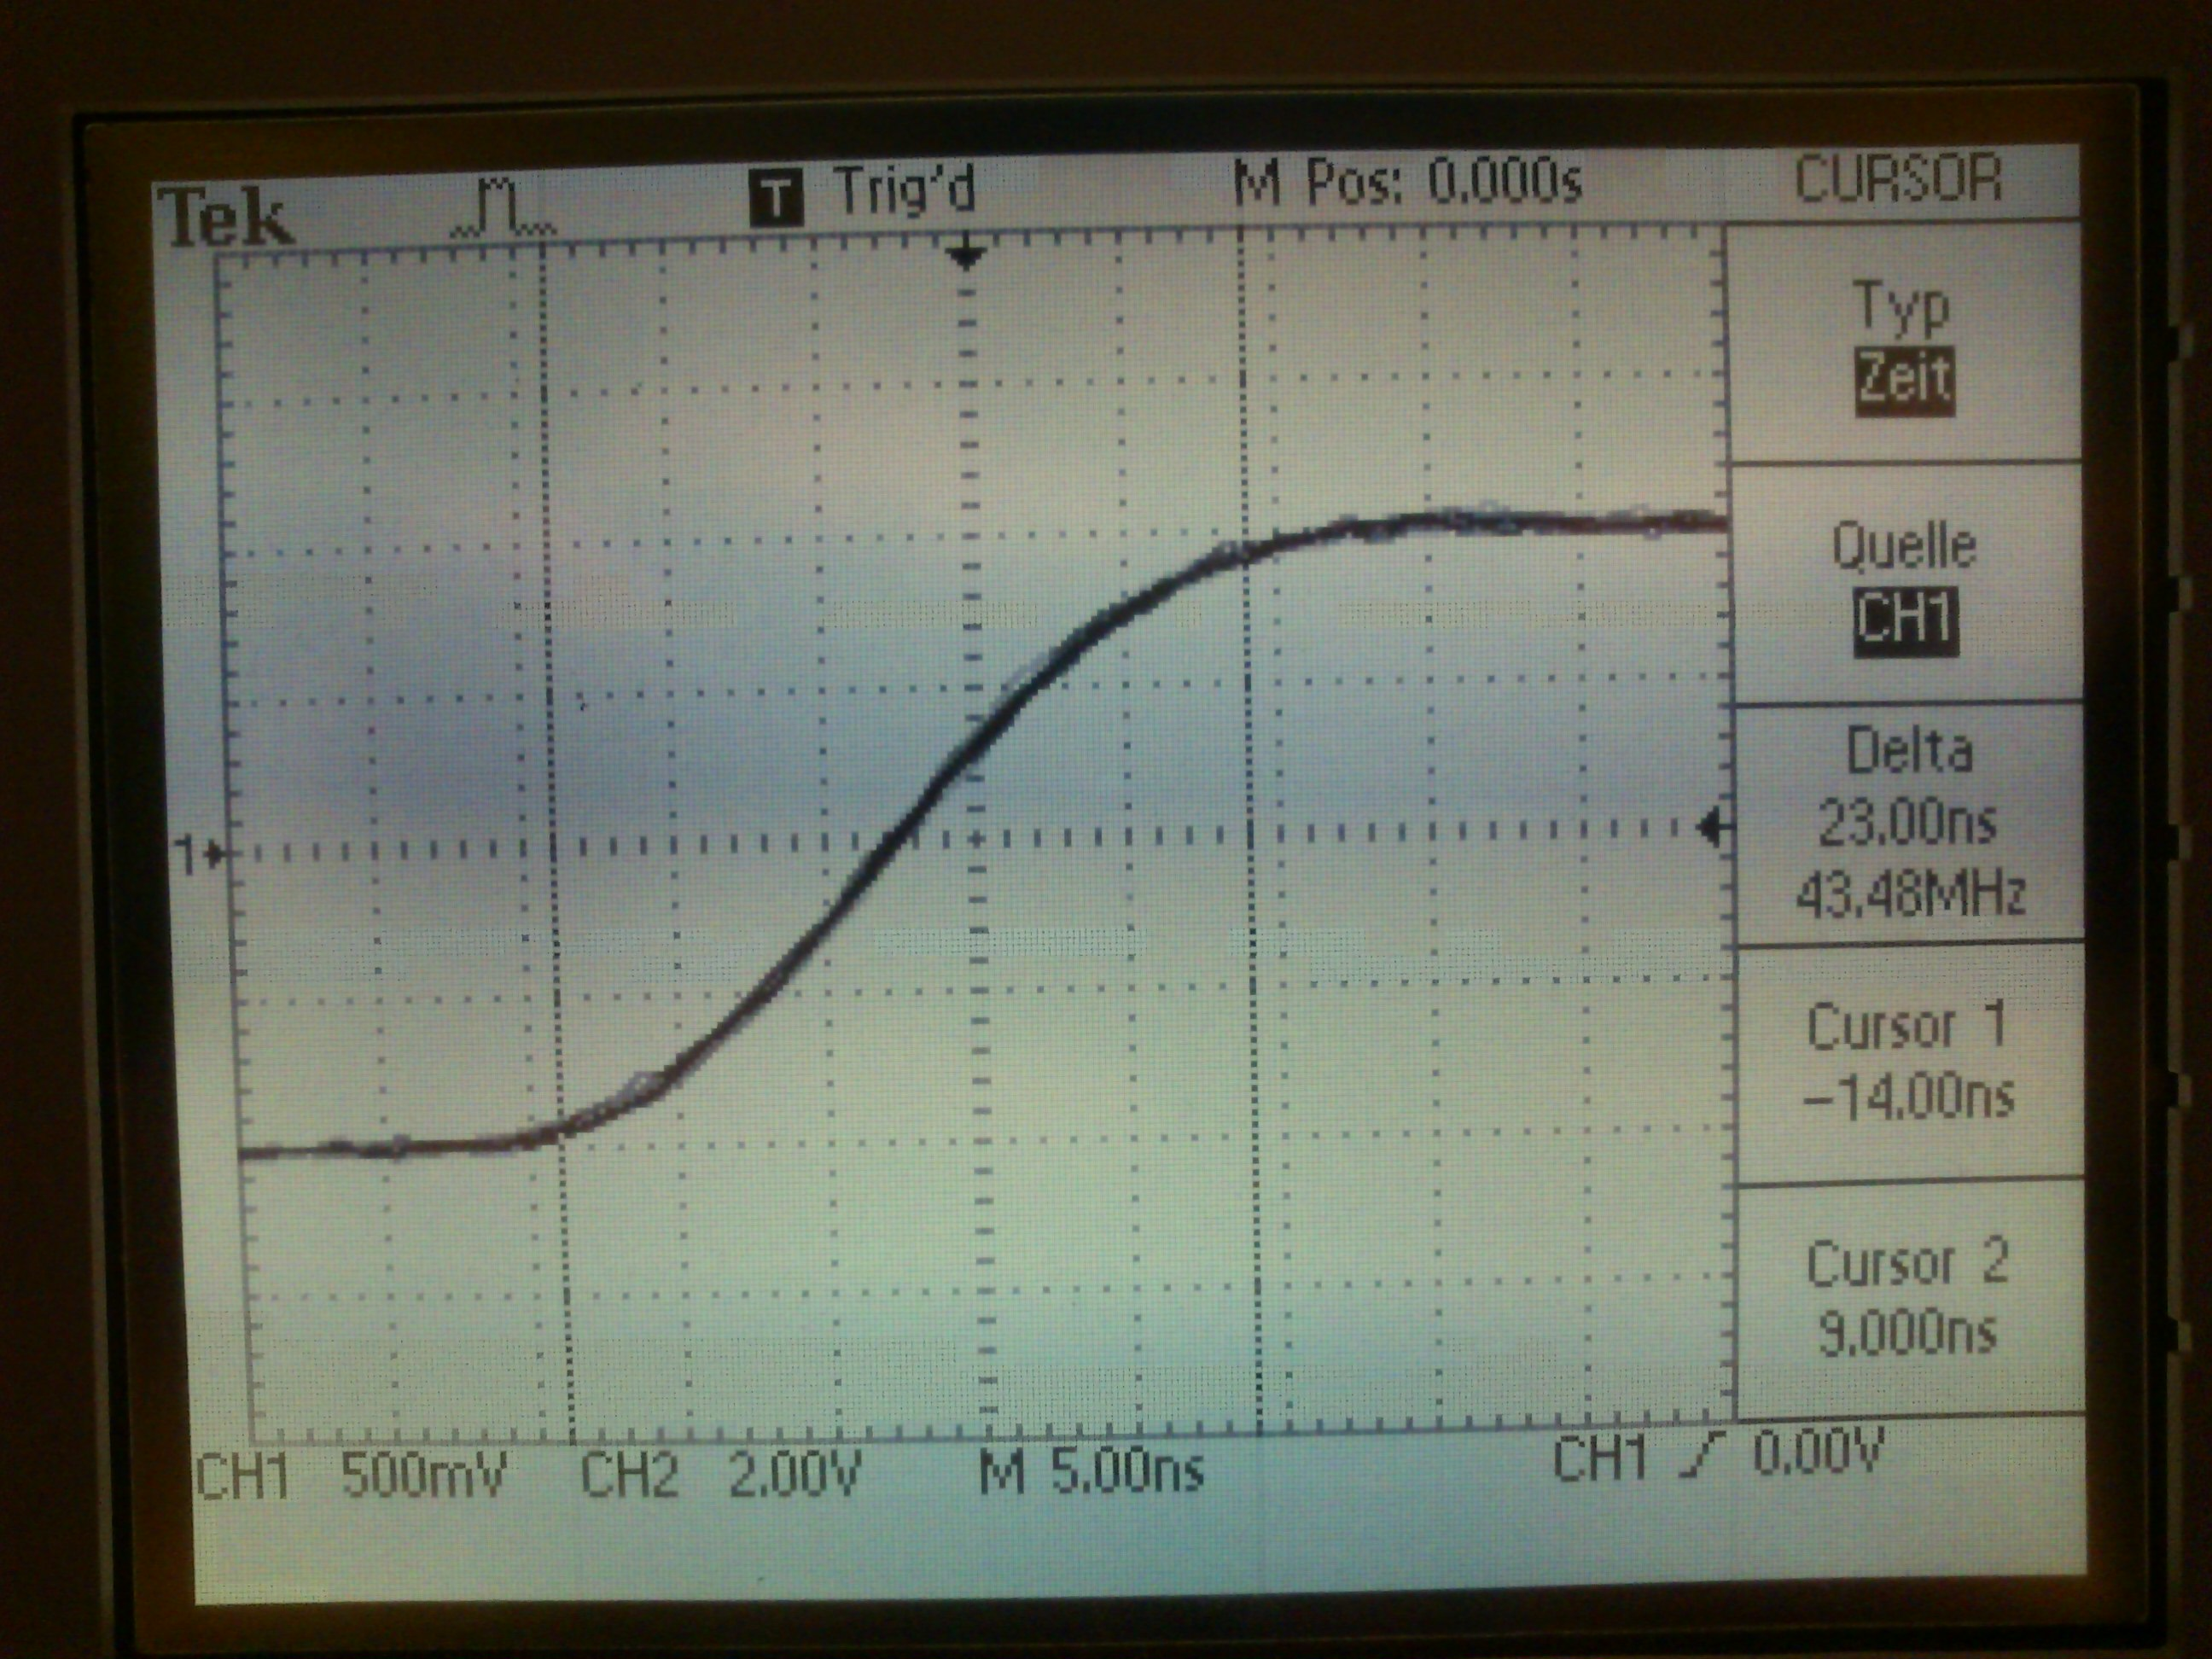
\includegraphics[width=\linewidth]{versuch3/oszi/DSC_0318.JPG}
	\caption{Messung der Anstiegszeit der normalen Rechteckspannung des Funktionsgenerators}
\end{figure}
Damit kann man die Bandbreite des Signals unter Berücksichtigung der Eigenanstiegszeit des Oszilloskops, die zuvor bestimmt wurde, berechnen:
$ t_{sig} = \sqrt{t_{ges}^2 - t_{oszi}^2} = \sqrt{23ns^2 - 2.6533ns^2} = 22.957ns $







%}}}

%}}}
